\chapter{Event reconstruction}
\label{chap:reco}

This chapter describes the reconstruction of events collected by the CMS
detector. The $\PH \to \Pgt\Pgt$ analysis requires almost every object measured in
CMS and makes use of information from every subdetector. The reconstruction of
each of these objects is summarised, followed by a description of a likelihood based
reconstruction of the di-tau mass. 

%Section \ref{sec:vertex} describes the reconstruction of the
%primary vertex using measured tracks in the event. Sections \ref{sec:electrons}
%and \ref{sec:muons} describe the reconstruction of the electrons and muons in
%the event combining the tracks with information from the \ac{ECAL} and muon
%chambers respectively. Section \ref{sec:jets} describes the reconstruction and
%treatment of jets, followed by section \ref{sec:met} describing how the missing
%energy of the event is computed. The reconstruction of hadronic taus
%is described in section \ref{sec:taus}.

%In addition to the reconstruction of the objects used in the $\PH \to \Pgt\Pgt$
%analysis, the final section of this chapter contains a description of a tool of
%great importance to this analysis - a likelihood based reconstruction of the
%di-tau pair mass, described in section \ref{sec:svfit}.

\section{Primary Vertex reconstruction}
\label{sec:vertex}
%Consider adding track reconstruction here too.

As discussed in section~\ref{sec:theLHC}, in the high instantaneous luminosity
conditions at the LHC there is a large probability for multiple proton-proton
collisions occurring in each bunch crossing. 
The reconstruction of the \ac{PV} of the event allows the identification of the hard
$pp$ interaction amongst other vertices due to such additional collisions. 
It also provides distinction between ``prompt" particles, i.e. production at the \ac{PV} from the hard
interaction, and in-flight decays of hadrons or photon conversions which occur
after the hard interaction.  

The vertices are reconstructed using the tracks collected in the inner
tracker. A clustering algorithm, \ac{DA}
\cite{DetAnnealing}, is used to assign tracks to their most likely 
vertex. Each vertex is seeded by at least two tracks separated in $z$ by less than
$1\,\cm$ at the point of closest approach to the $z$ axis.
The most likely position of each vertex is then determined using the
adaptive vertex fitter \cite{adaptivevertex}. In
this algorithm each track is assigned a weight, $w_{i}$, which is close to one for tracks which
are highly compatible with the fitted vertex position and close to zero for tracks with low
compatibility. These weights are used to define the number of degrees of freedom
for the fit: $n_{\text{dof}}^{\text{vertex}} = 2\sum_{i}^{\text{tracks}}w_{i}-3$. This
variable is an assessment of the mutual compatibility of the component tracks of
the vertex, and is used to distinguish real $pp$ interactions from
misreconstructed vertices. For most analyses, the following quality cuts are
applied on each vertex~\cite{CMS-PAS-TRK-10-005}:
\begin{itemize}
\item The distance in the $z$ direction from the vertex to the nominal interaction
point must be smaller than $24\,\cm$. 
\item The corresponding distance in the transverse plane must be smaller than
$2\,\cm$.
\item $n_{\text{dof}}^{\text{vertex}} > 4$.
\end{itemize}

The \ac{PV} is taken to be the vertex with the highest sum squared transverse
momentum ($\pt$) of its associated tracks. 

\section{Electrons}
\label{sec:electrons}

Electrons are reconstructed by matching \ac{ECAL} deposits with tracks from the
inner tracker. This is made more difficult by the electrons
undergoing bremsstrahlung when interacting with the material of the tracker.
The photons produced can also convert to $\Pep\Pem$ pairs before
reaching the \ac{ECAL}. This means that the energy deposited in the \ac{ECAL} 
can be spread out in the $\phi$ direction. Hence dedicated algorithms are used
to combine the energy deposits from both the initial electron and the
bremsstrahlung products, known as ``supercluster'' algorithms \cite{ElectronReco}.

Separate algorithms are used for electrons in the barrel and endcaps, in
order to be optimal for the different geometries. In both cases, a clustering is performed
in the $\eta$--$\phi$ plane starting from the \ac{ECAL} crystal with the most energetic deposit, and
continuing outwards to the surrounding crystals until there are no more
unclustered crystals above a certain energy threshold. In the barrel, the
``hybrid'' clustering algorithm is used. In this algorithm the seed crystal
has $\Et>1\,\GeV$ and the clustering is performed in a ``domino'' of $3\times1$ or
$5\times1$ crystals, with additional dominoes (which attempt to collect
radiation deposits) stepping in both $\phi$
directions around the seed up to $\Delta\phi\approx0.3$. The energy threshold
below which crystals are not clustered  is $100\,\MeV$. In the endcaps the
approach is similar with a clustering algorithm
called the ``Multi5$\times$5'' algorithm using $5\times5$ arrays of crystals within
$\Delta\eta<0.07$ and $\Delta\phi<0.3$~\cite{CMS:2013hoa}.

The energy-weighted average position of the supercluster is computed, which
is the equivalent of the impact point in the \ac{ECAL} of a
non-radiating electron with energy equal to the supercluster energy. This is
matched to a compatible hit in a loose $\phi$--$z$ search region 
in the first pixel layer, under the
hypothesis that the electron could be either charge. If a compatible hit is
found, the hit in the first layer is used to update the estimated electron
trajectory which would result in hits in the outer layers. This seeds the
reconstruction of the electron trajectory through the tracker
using the \ac{GSF} algorithm~\cite{GSFalgorithm}. This provides an additional momentum measurement
which is used to improve the electron energy resolution. 

%Backgrounds to electrons are expected to originate
%in hadronic jets, for example where a $\Pgpz$ and $\Pgppm$ overlap, or where a
%$\Pgppm$ showers early in the \ac{ECAL}.
% read the paper and understand better what these backgrounds are!! pions?
Electron identification (ID) criteria are used in many analyses to improve the efficiency of
selecting real electrons over backgrounds which tend to originate from
hadronic jets. The most commonly used variables are \cite{Baffioni:2006cd}:

\begin{itemize}
\item $\Delta\eta_{in}$ and $\Delta\phi_{in}$, the separation in the
$\eta$ and $\phi$ between the supercluster and track direction
evaluated at the \ac{PV} position and extrapolated to the \ac{ECAL} (generally
smaller for prompt electrons).
\item $\sigma_{\eta\eta}$, the energy-weighted $\eta$ width of the cluster.
This is typically small for prompt electrons, which have a more localised
cluster.
\item $H/E$, the ratio of hadronic to electromagnetic (EM) energy in the region of
the seed cluster. This is also generally lower for prompt electrons.
\end{itemize}

Figure \ref{fig:electronID} shows the distributions of these variables in both simulated
electrons and backgrounds from jets in the barrel.

\begin{figure}
\begin{center}
\subfloat[]{
    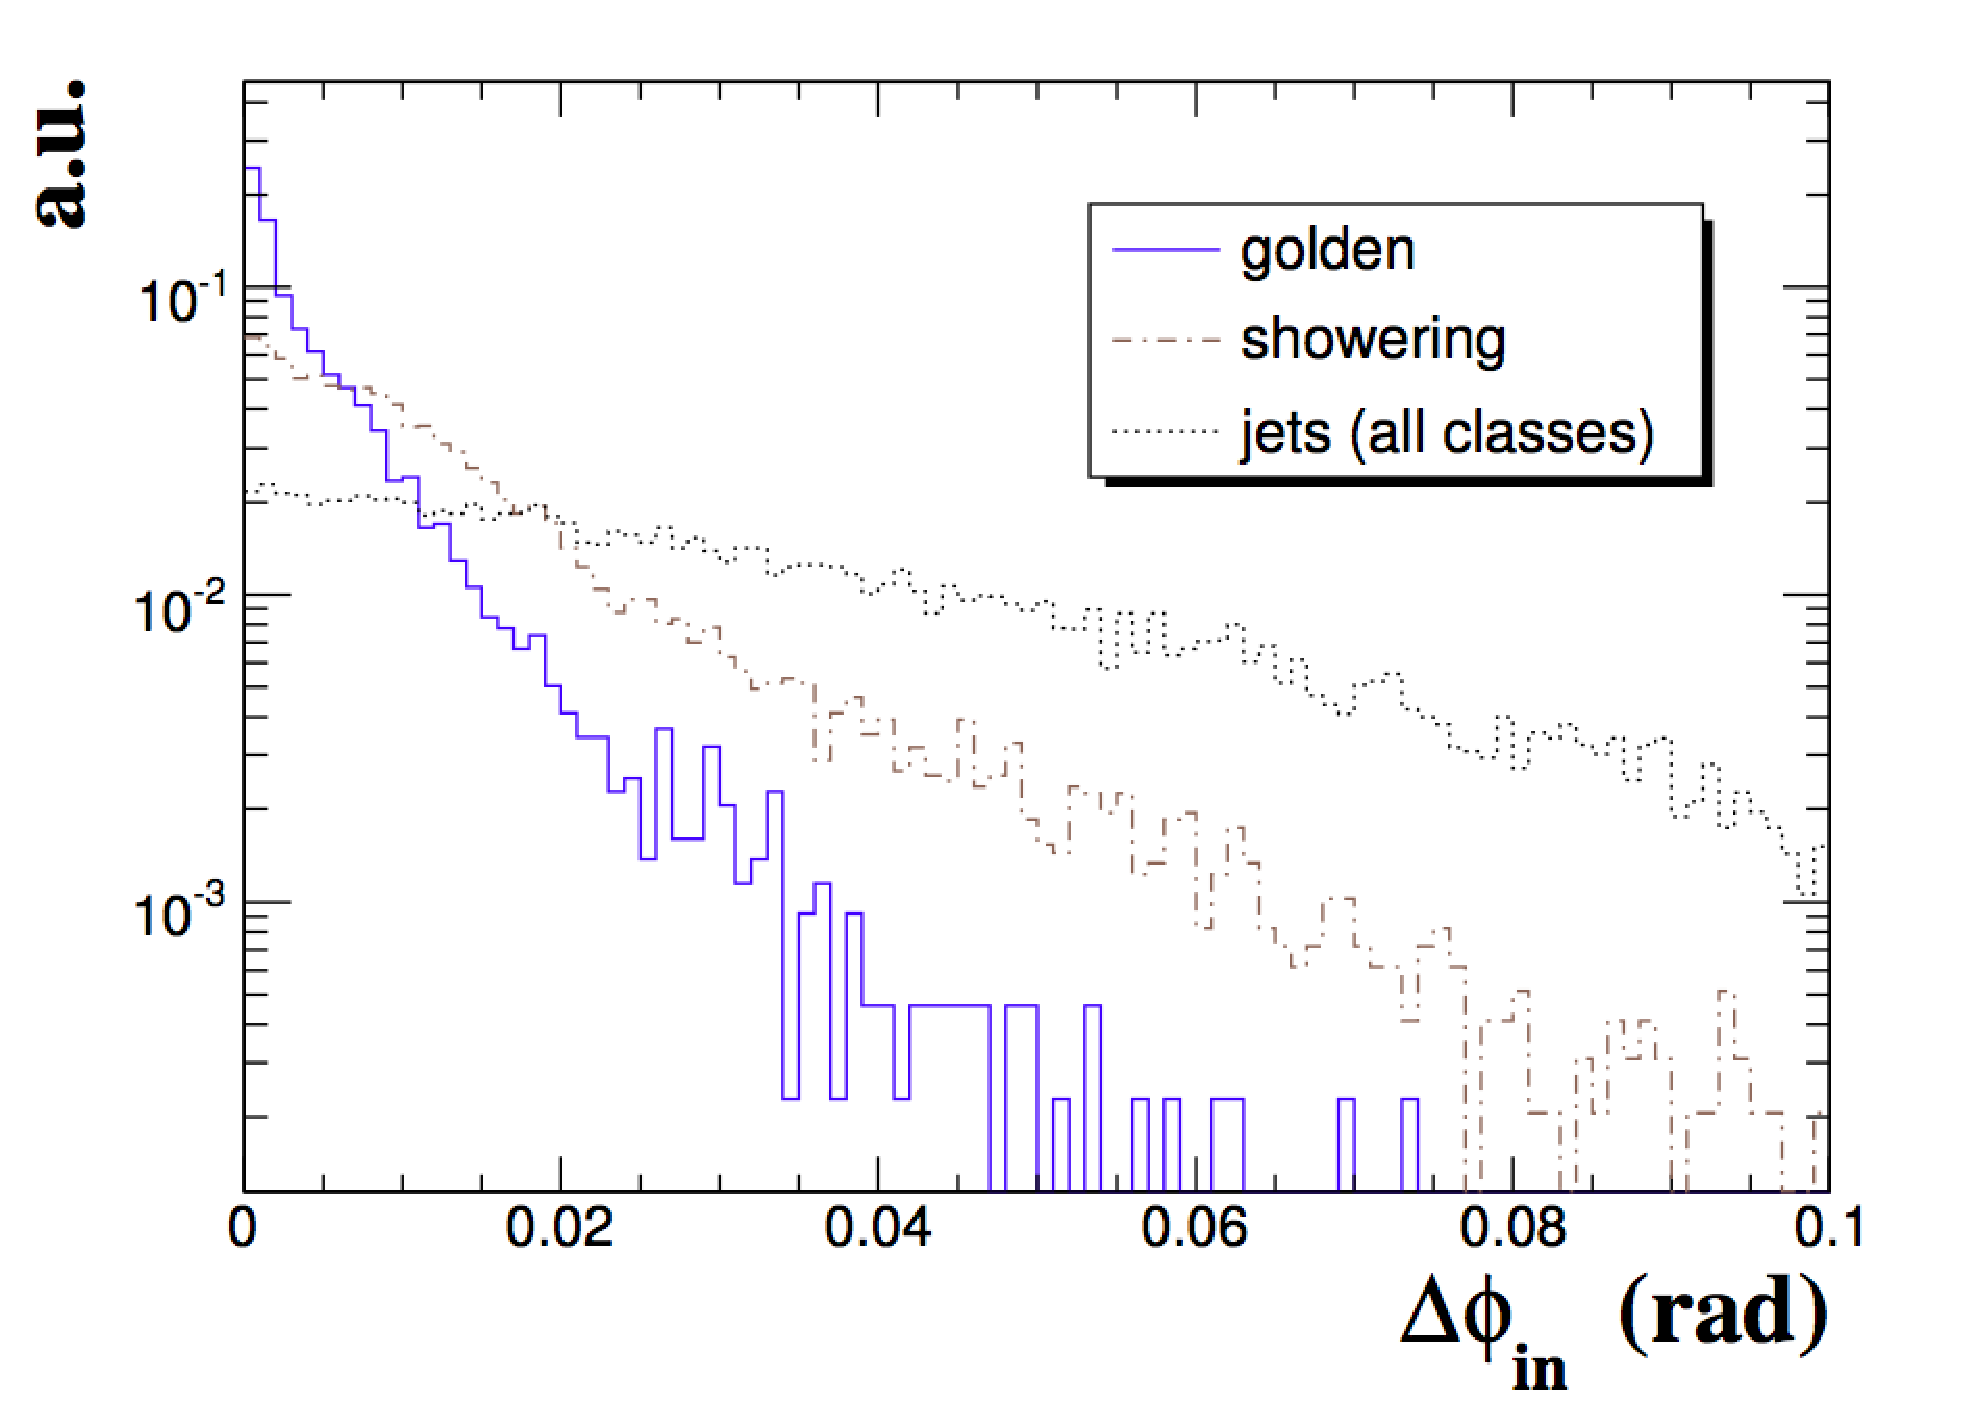
\includegraphics[width=0.5\textwidth]
      {plots/reco/elec-dphi.pdf}}
\subfloat[]{
    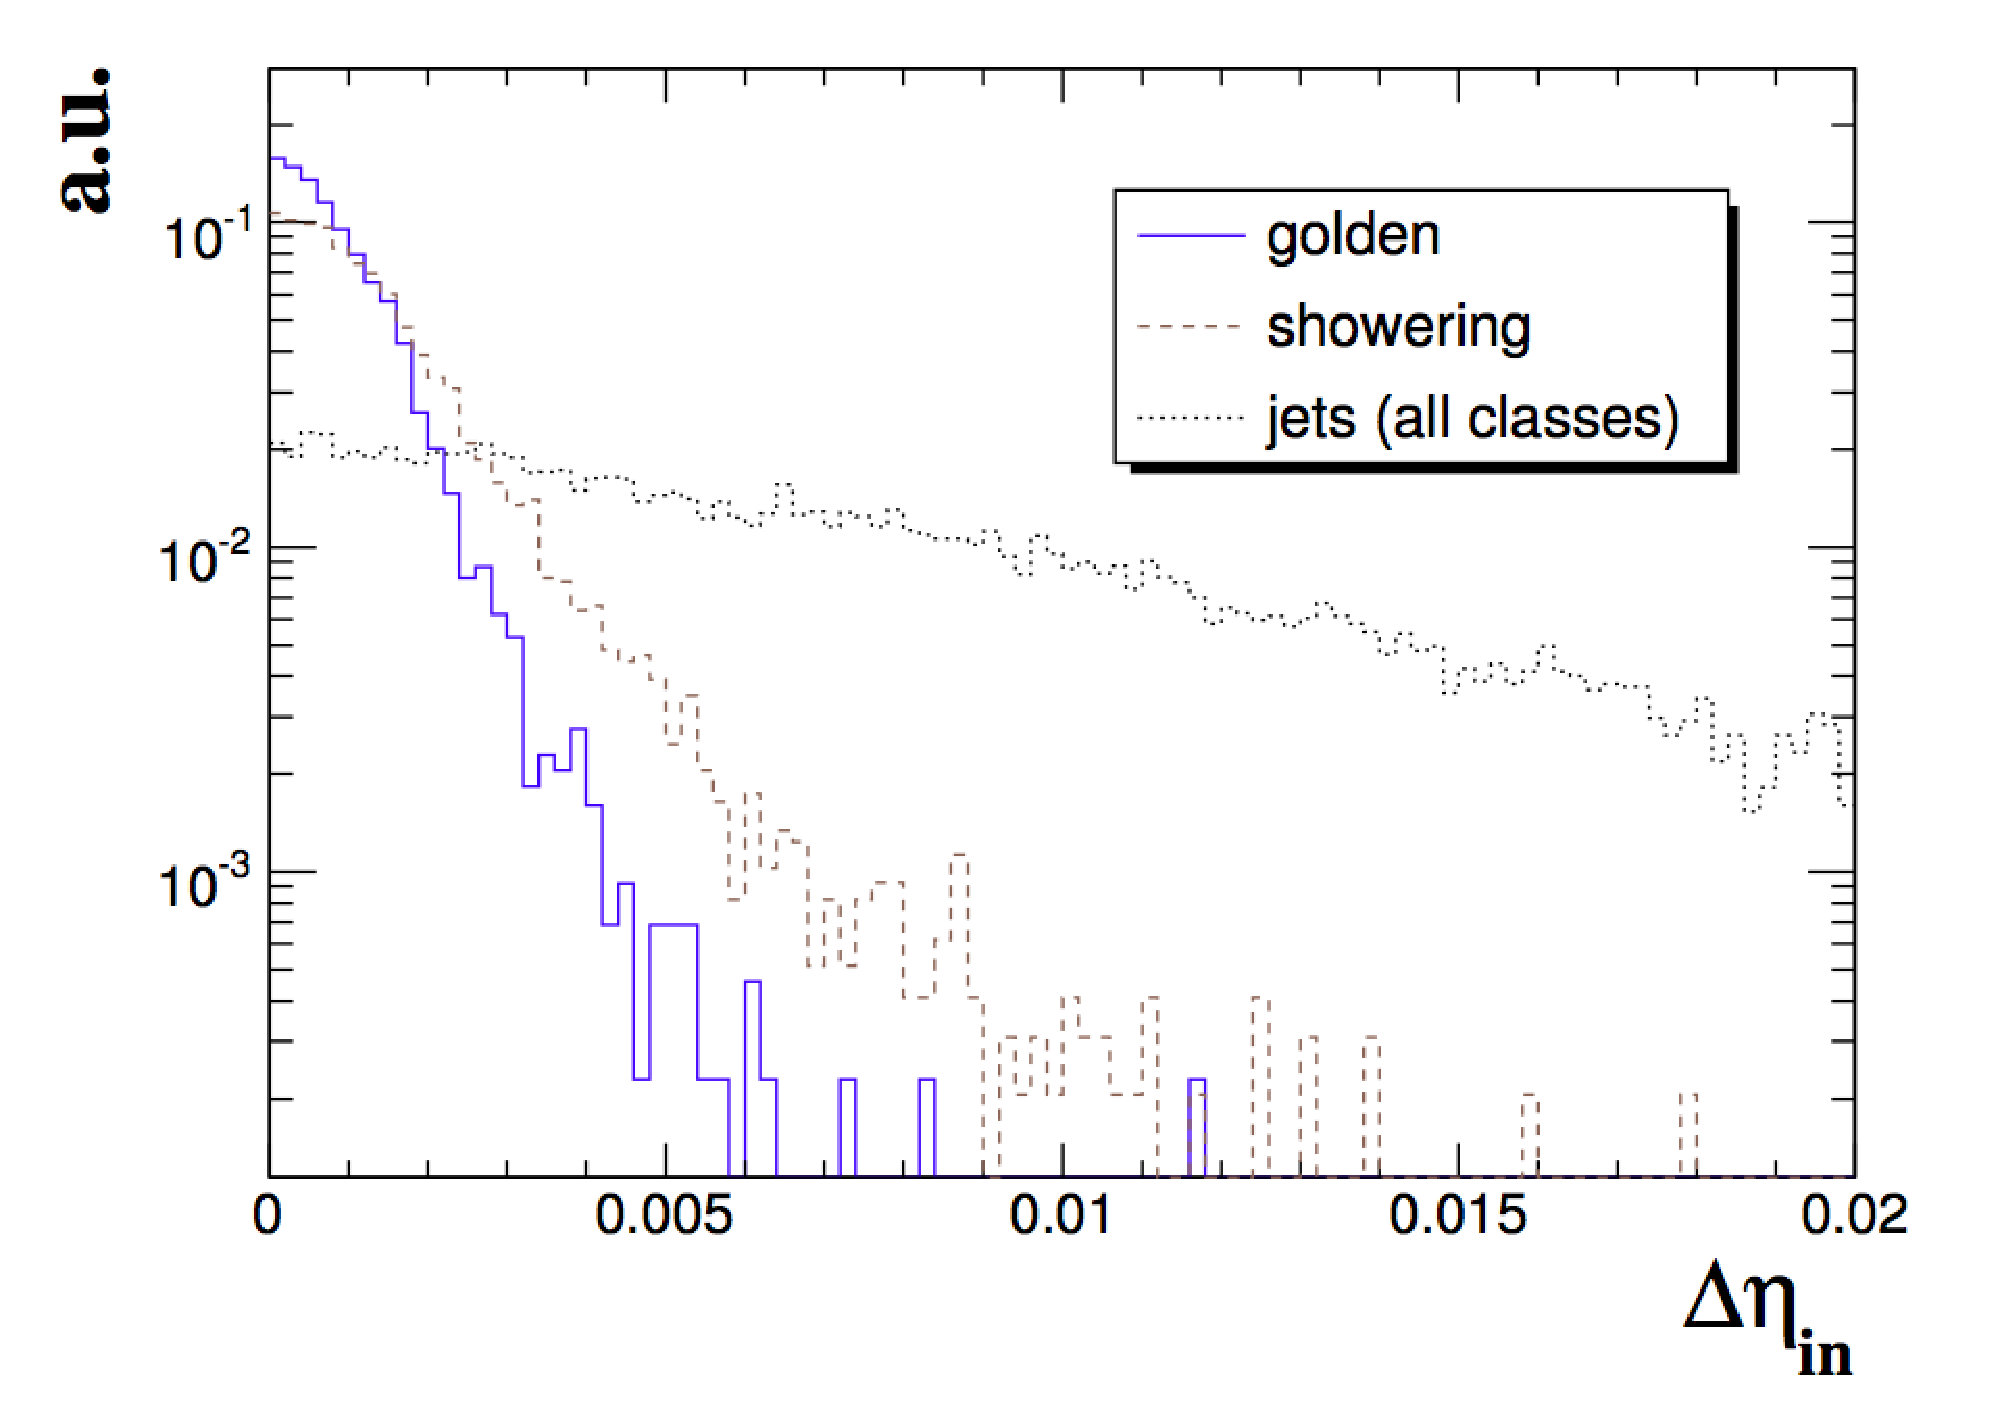
\includegraphics[width=0.5\textwidth] 
      {plots/reco/elec-deta.pdf}} 

\subfloat[]{
    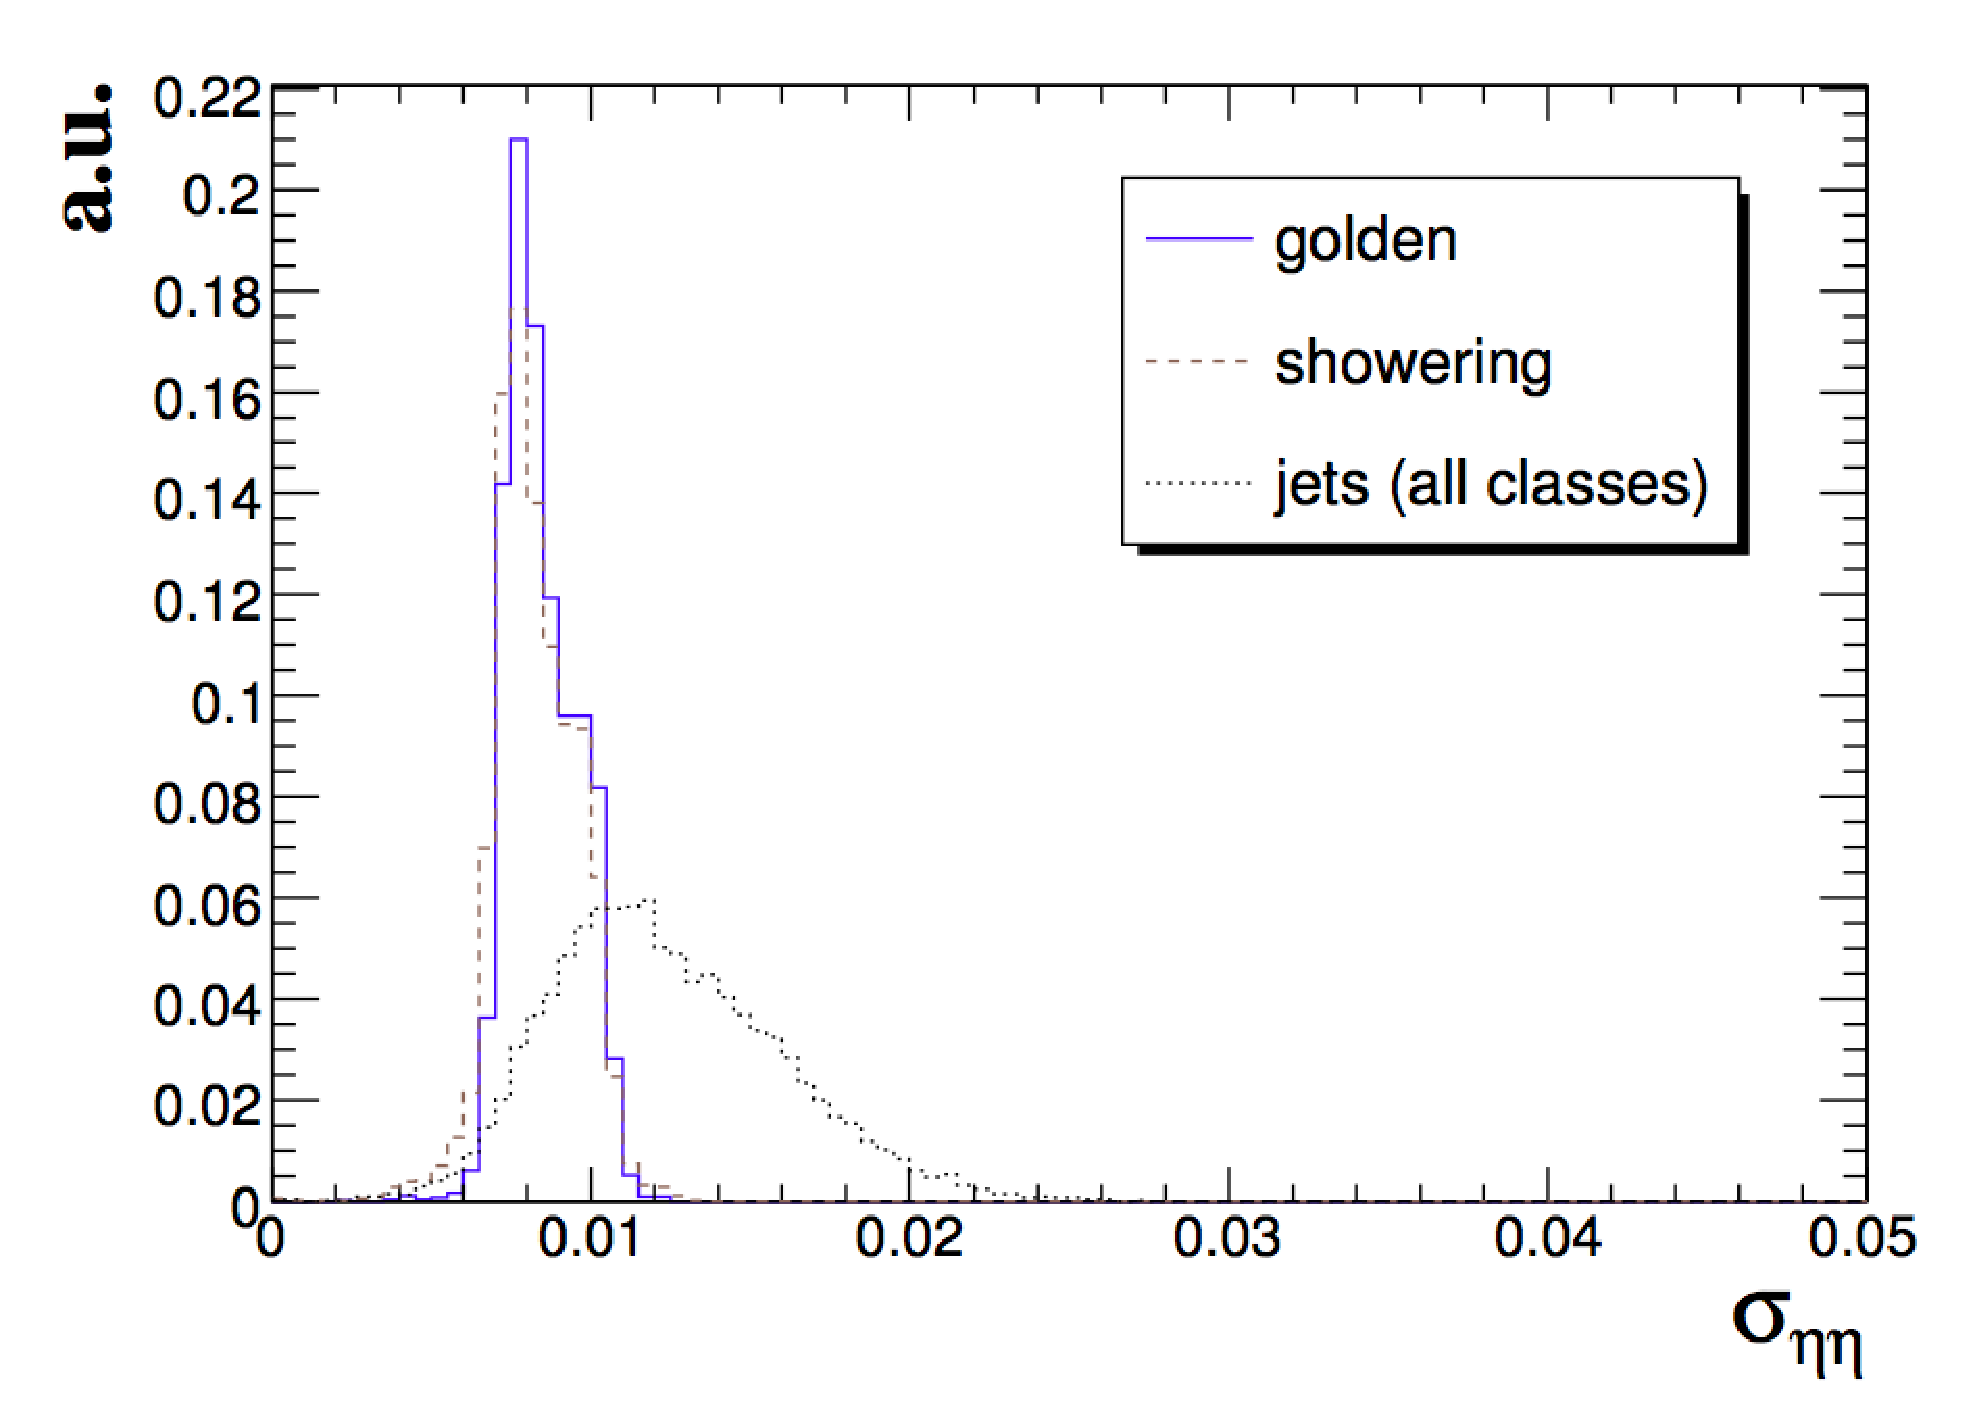
\includegraphics[width=0.5\textwidth]
      {plots/reco/elec-sigieie.pdf}}
\subfloat[]{
    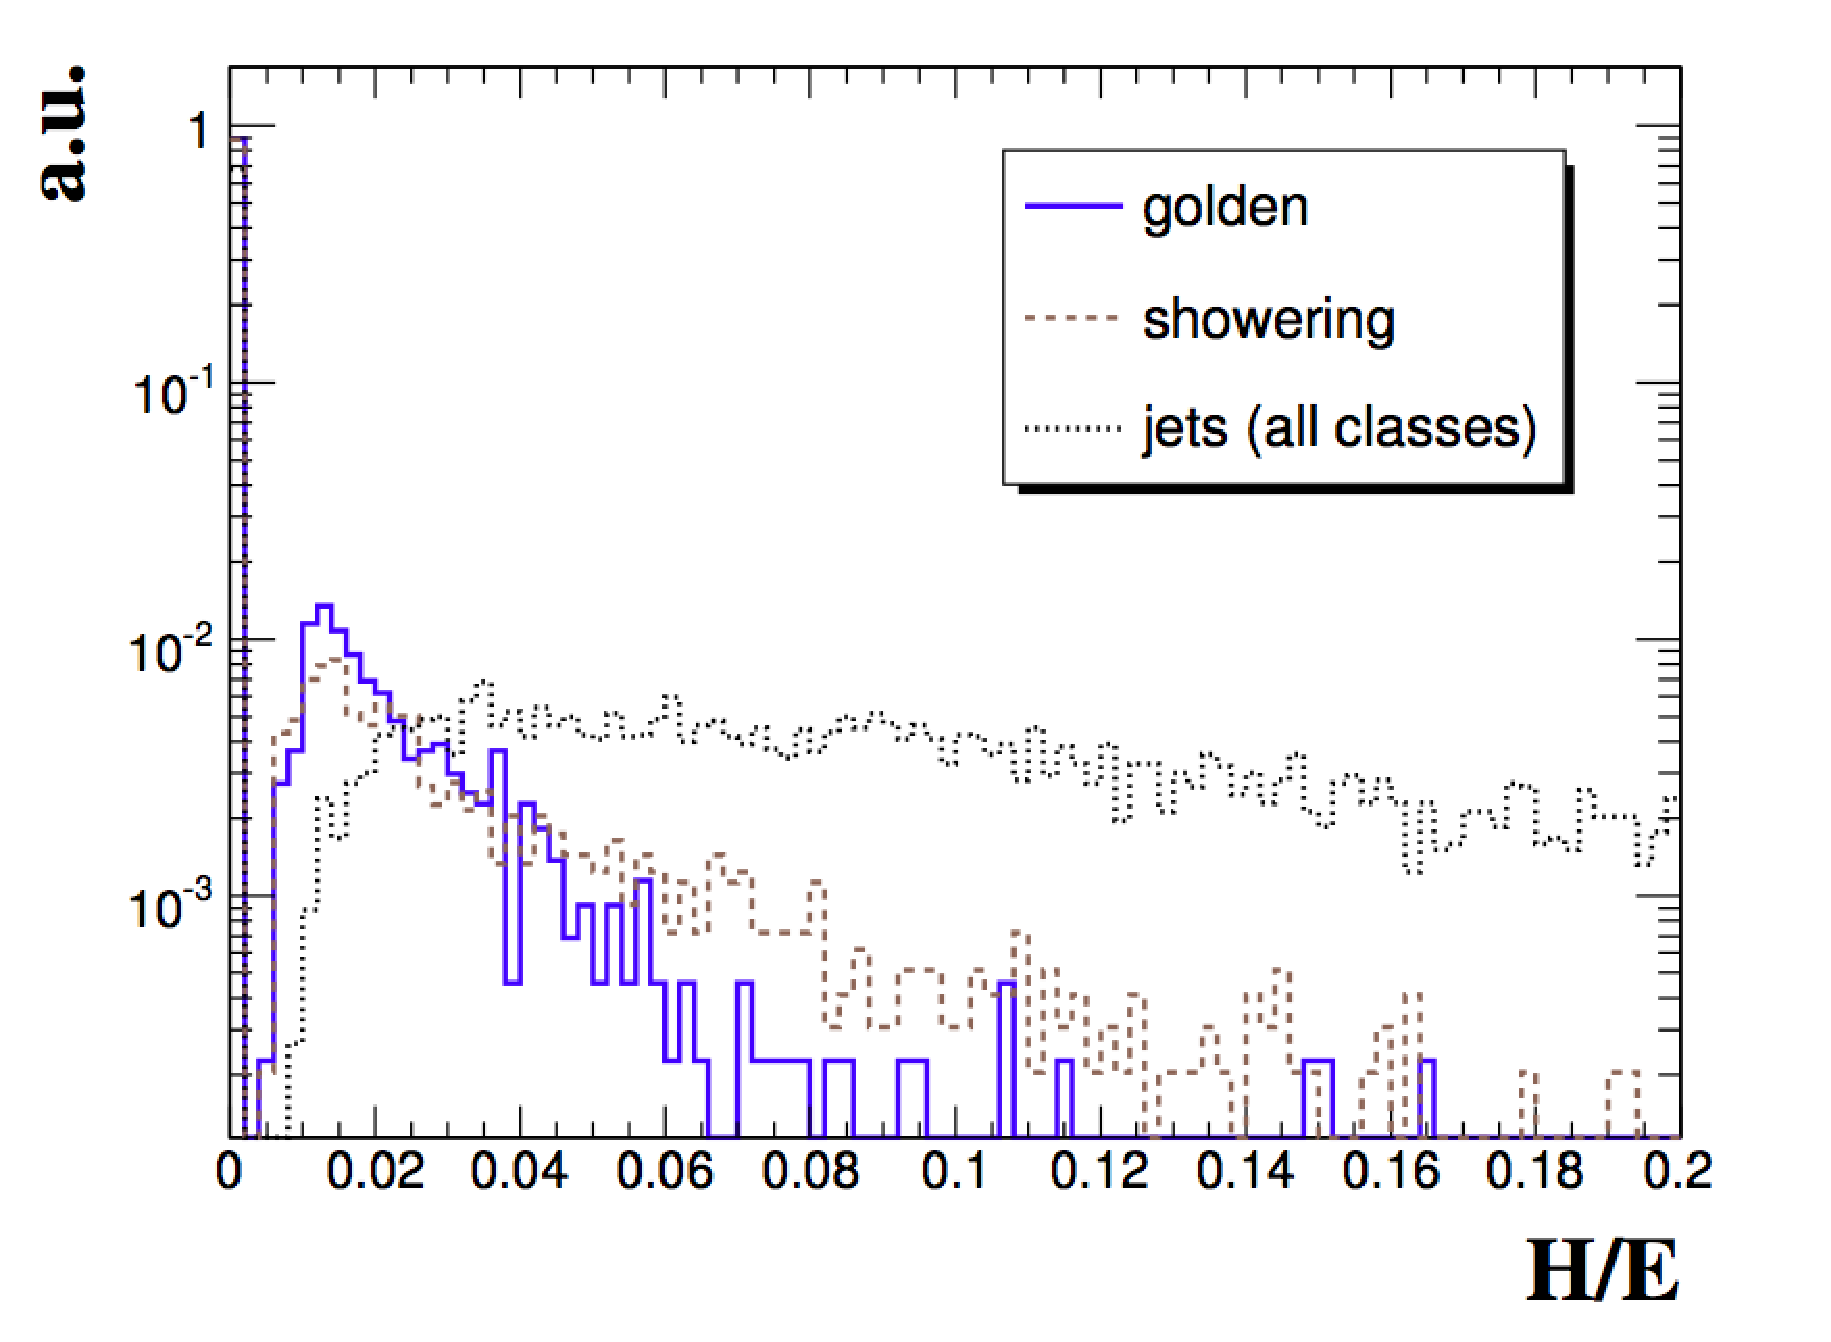
\includegraphics[width=0.5\textwidth]
      {plots/reco/elec-HE.pdf}} 
\end{center}
\caption[Distributions of variables related to the electron supercluster in the
ECAL.]{
    Distributions showing: the separation in a) $\phi$ and b) $\eta$ between the supercluster and the
    track direction, c) the energy-weighted $\eta$ width of the cluster and d)
    the ratio of hadronic and electromagnetic energy in the region of the seed
    cluster. Shown for electrons and backgrounds from jets \cite{Baffioni:2006cd}. 
}
\label{fig:electronID}
\end{figure} 

The electron ID used in the $\PH \to \Pgt\Pgt$ analysis makes use of these four variables and additional
conditions on the track quality and kinematics~\cite{Baffioni:2006cd} to provide
improved ID efficiency. These variables are combined in a
multivariate \ac{BDT}~\cite{TMVA}, which is trained in two bins of
$\pt$ and three bins of $\eta$ using $Z/\gamma^{*} \to \Pe\Pe$ events in
data.
The additional variables used as inputs to the \ac{BDT} are:

\begin{itemize}
\item Quantities relating to the quality of the tracks, including the normalised
$\chi^{2}$ and the number of valid hits in the track fit.
\item Additional quantities relating to the cluster shape, including the
variable $f_{e}=1-e_{1\times5}/e_{5\times5}$, in which $e_{1\times5}$
($e_{5\times5}$) denotes the energy deposited in an array of $1 \times 5$ ($5
\times 5$) cells in the vicinity of the supercluster seed, and the variable
$R_{9}$, which gives the fraction of the supercluster energy in an array of
$3\times3$ cells in the vicinity of the supercluster seed.  
\item Additional variables relating to the compatibility of the hadronic and EM
energy with the track momentum, including the ratio of supercluster energy over
the momentum of the associated track evaluated at the \ac{PV} (E/P), the
quantity $1/E-1/p$ which quantifies the energy-momentum compatibility, the ratio
of the electron cluster energy to the momentum of the associated track evaluated
at the surface of the calorimeter and the ratio of the energy reconstructed in
the pre-shower detector over the raw energy of the supercluster.  
\end{itemize}

The \ac{BDT} output is a $\pt$ and $\eta$ dependent cut threshold. Finally
non-prompt electrons from photons interacting with the tracker are suppressed
by requiring there are no missing hits in the inner tracker and that the
electron is not matched to a reconstructed conversion. The electron must also be
consistent with the \ac{PV}, by having small impact parameters. Studies
of the efficiency of the electron ID in the $\PH \to \Pgt\Pgt$ analysis can be
found in section \ref{sec:datamcfactors}.

\section{Muons}
\label{sec:muons}

Muons typically travel through the CMS calorimeters with minimal energy deposit
and are reconstructed in the muon chambers. Thus muons can be reconstructed
in two independent places - the tracker and the muon chambers. This
greatly improves the ability to isolate muons from hadronic activity. The
``global'' muon reconstruction algorithm~\cite{MuonReco} uses both sets of information by
starting from each track in the muon chambers and searching for a compatible
track in the inner tracker. If a compatible track is found, the energy and
momentum of the muon is determined by a fit to the hits in both the inner
tracker and the muon chambers, taking into account the expected energy loss
within the magnet. This improves the momentum resolution compared to
the track only measurement for muons with $\pt$ larger than $200\,\GeV$. For
lower $\pt$ muons, the momentum resolution is driven by the fit to the tracker
hits. For muons with $\pt < 5\,\GeV$, the reconstruction starting from the inner
tracker is more efficient due to the lower probability of these muons reaching
the muon chambers. This is known as ``tracker'' muon reconstruction.  

Backgrounds to prompt muons consist of non-prompt muons from in-flight decays of
hadrons and ``punch-through'' of charged hadrons which pass through the calorimeters
into the muon chambers. These backgrounds are reduced through the use of ID
requirements based on the properties of the muon track. In flight decays are
reduced by the requirement of hits in at least one pixel detector and $5$
tracking layers. The $\chi^{2}$ of the global track fit must be better than
$10$, and the global track fit must include hits from at least one segment in
the muon detector, both of which provide rejection of punch-through hadrons. In
addition, track segments must be found in at least two stations of the muon
detector. These conditions taken together provide the ``tight'' muon ID used in
many analyses, including the $\PH\to\Pgt\Pgt$ analysis.
The efficiency of CMS muon reconstruction is found to be better
than $96\%$ for muons with $\pt > 10\,\GeV$~\cite{MuonReco}. Studies of the ID efficiency of
muons in data and \ac{MC} in the context of the $\PH \to \Pgt\Pgt$ analysis can
be found in section \ref{sec:datamcfactors}.

\section{Lepton isolation}
\label{sec:leptonisolation}

In order to further reduce background contributions from misidentified QCD jets,
electrons and muons are required to be isolated~\cite{CMS:2013hoa,MuonReco}. 
Isolation is computed as the scalar sum of transverse momenta of the particles within a cone in
$\eta$--$\phi$ space of size $\Delta R = 0.4$ centred on the lepton direction. 
This sum includes all charged particles, neutral hadrons and photon candidates. 
To reduce the contamination of particles which originate from \ac{PU} events 
in this cone, charged  candidates with an impact parameter greater than 
$0.1\,\cm$ from the primary vertex are excluded from the sum. An estimate of the 
neutral pileup contribution is made based on the charged pileup contamination,
multiplied by a factor 0.5, which is approximately the ratio of neutral to
charged components of the hadronisation, as determined from simulation.   
The isolation is then defined as follows:

\begin{equation}
I = \sum^{\substack{\text{charged} \\ \text{non-pileup}}}\pT +
\text{max}\left(0,\sum^{\text{neutral}}\pT+\sum^{\text{photon}}\pT-\frac{1}{2}\sum^{\substack{\text{charged}
\\ \text{pileup}}}\pT\right).
\label{eq:leptonisolation}
\end{equation}

Requirements are usually placed on relative isolation, defined as
$I_{\text{rel}} = I / \pt^{\text{lepton}}$. 

\section{Jets}
\label{sec:jets}

Jets result from the large numbers of quarks and gluons present in a hadron
collider. The term `jet' is used to refer to the collimated shower of particles
which is produced from the hadronisation of a quark or gluon. In order to
reconstruct the original parton, these showers of particles are collected
and combined. 
%Before describing exactly how this is done, section
%\ref{sec:particleflow} describes an important algorithm which greatly improves
%this reconstruction. 

\subsection{Particle flow}
\label{sec:particleflow}

CMS uses a \ac{PF} \cite{CMS-PAS-PFT-09-001,CMS-PAS-PFT-10-001,CMS-PAS-PFT-10-002} 
algorithm to combine the individual track and energy deposits in each sub-detector. 
This allows the reconstruction of individual particles emerging from all vertices: charged
hadrons, neutral hadrons, photons and the muons and electrons already discussed.
These particles can then be 
used to calculate the missing transverse energy $\MET$,
reconstruct jets and quantify the isolation of leptons and photons. A separate
algorithm is used to reconstruct hadronic decays of taus, discussed in section
\ref{sec:taus}. The \ac{PF} algorithm combines the high resolution of
the tracker with the energy resolution and high granularity of the calorimeters.

The output of the \ac{PF} algorithm is a set of the stable particles in the event
resulting from the hard interaction, from the inputs of charged particle tracks,
calorimeter energy deposits and muon chamber hits. The clustering of energy
deposits is performed separately in the \ac{ECAL} and \ac{HCAL}. For electrons
as discussed in section \ref{sec:electrons} this allows the combination of
bremsstrahlung photons with the parent electrons and in the \ac{HCAL} this
allows the separation of the neutral and charged hadrons. The clustering
proceeds by first defining a cluster seed, which corresponds to the calorimeter
cell with the highest local energy. The threshold for clustering neighbouring
cells is that they must have energy greater than 2 standard deviations above
noise level. After the clustering, the different \ac{PF} elements are linked into
blocks to be interpreted as a particular particle. This can be done using
extrapolation of tracks into the calorimeters, where the two elements are linked
if the track falls inside the cluster volume.

\subsection{Jet identification by clustering}
\label{sec:jetID}

Jets can be composed of many sub-particles, which may interact in the detector
in different ways. These particles must be combined using a clustering
algorithm~\cite{Salam:2009jx}, where the choice of algorithm defines how the particles should be combined
taking into account the distance between the objects. In particular the
algorithm should be infrared- and collinear- safe, meaning that the jet
reconstruction is not affected by soft QCD radiation or gluon splitting.
The algorithm used for the $\PH\to\Pgt\Pgt$ analysis is the
`anti-$k_{\text{T}}$' algorithm~\cite{Cacciari:2008gp} as implemented in
the \textsc{fastjet} package~\cite{Cacciari:fastjet1}, which considers all 
objects within a certain jet `size' defined by a parameter $R=0.5$, and 
sequentially combines them starting from the one with the
smallest distance from the beamline. If this distance is smaller than the
distance between this object and the closest second object then the first is
taken to be a final state jet and removed from the object list,
otherwise the two objects are combined into one and the process repeats. 
This process is repeated for all objects until none remain in the list. The effect of this
is to form a cluster around the hardest particles in a cone in $\eta$-$\phi$.

Jet identification criteria are applied to reduce the contribution of jets from
noise in the calorimeters. These include the following:
\begin{itemize}
\item Jets must consist of at least one \ac{PF} component. 
\item The jet energy must have contributions
from both the \ac{ECAL} and \ac{HCAL} (above a given noise threshold).
\item The fraction of the total jet energy as a result of photons or neutral
hadrons should be less than 0.99 of the total jet energy.
\item Jets within the acceptance of the inner tracker must have at least one
charged object and a charged energy fraction greater than zero and an electron
energy fraction less than 0.99. 
\end{itemize}

\subsection{Jet energy corrections}
\label{sec:JEC}

An important aspect of jet identification is the correct measurement of the jet
energy, which is typically different between reconstructed and true hadron-level jet energy
due to experimental effects. This can be due to uninstrumented regions of the
detector, non-linear calorimeter response and contamination by jets from \ac{PU}
interactions. Particles from different \ac{PU} vertices can be clustered and identified as a
jet, or overlap with a jet from the primary vertex affecting the measurement of the jet energy.
Pileup jet identification \cite{CMS-PAS-JME-13-005} is used to classify these events, which uses a 
\ac{BDT}~\cite{TMVA} with input variables such as
momentum and spatial distribution of the jet particles. In addition
a calibration factor is applied to account for imperfections in the
neutral-hadron calibration, the jet energy containment and small differences
between the simulated and observed response.

To account for the detector effects and remaining \ac{PU}, a correction to the jet energy
scale is derived~\cite{CMS-JME-10-011}:

%Read this paper when you have internet and find a better way to write this
%equation

\begin{equation}
P_{\text{corr}}^{\mu} = C_{\text{PU}}(\pT^{\text{raw}},\eta) \cdot
C_{\text{rel}}(\pT^{\text{PU}},\eta) \cdot C_{\text{abs}}(\pT^{\text{rel}},\eta) \cdot
P_{\text{raw}}^{\mu}\, .
\end{equation}

In this equation, $C_{\text{PU}}$ is the correction for \ac{PU},
$C_{\text{rel}}$ is a relative correction and $C_{\text{abs}}$ is an absolute
correction. The corrections are applied sequentially such that the \ac{PU}
correction is a function of raw jet $\pt$ ($\pt^{\text{raw}}$),
the relative correction is a function
of the $\pt$ corrected for the pileup effects ($\pt^{\text{PU}}$) and finally
the absolute correction is a function of the relative-corrected $\pt$
($\pt^{\text{rel}}$). All of the corrections are applied as a function of
jet $\eta$. These subsequent corrections are applied to the raw
4-vector of the jet $P_{\text{raw}}^{\mu}$ to yield the corrected 4-vector
$P_{\text{corr}}^{\mu}$.

The \ac{PU} correction $C_{\text{PU}}$ is determined using the $\pt$ density in the event to
estimate the contribution from \ac{PU} on a per-jet basis. The relative
correction is determined using a dijet $\pt$ balance method which uses dijet
events containing a reference jet with $|\eta| < 1.3$ and exploits momentum conservation.
The probe jet (which can have any value of $\eta$), is used to calculate the
average of a balance quantity, defined as:
$(\pT^{\text{probe jet}}-\pT^{\text{ref jet}})/\pT^{\text{average}}$, in bins of
average dijet $\pt$ and probe $\eta$.  

The absolute correction is measured
using the \ac{MPF} method~\cite{Abe:1992sj}, using $\Pphoton$+jets and $\PZ$+jets
events and enforcing momentum conservation exploiting the fact that these
events shouldn't contain any real $\MET$. Thus any measured $\MET$ can be used to
calibrate the $\pt$ of the jets. The total uncertainty on the jet energy scale
is given by the sum in quadrature of the estimated uncertainties in each of the
correction factors. Figure~\ref{fig:jesuncert} shows the total value of the jet
energy scale correction factor for two different $\pt$ values for jets
reconstructed using the \ac{PF} algorithm and two other types also used at CMS.
Only \ac{PF} jets are used in the $\HToTauTau$ analysis and so the other two
types are not described in this thesis. The bands show the corresponding total jet 
energy scale uncertainty. The total uncertainty varies between approximately $3$ and 
$5\%$ depending on $\pt$ and $\eta$~\cite{CMS-JME-10-011}. 

\begin{figure}
\begin{center}
\subfloat[]{
    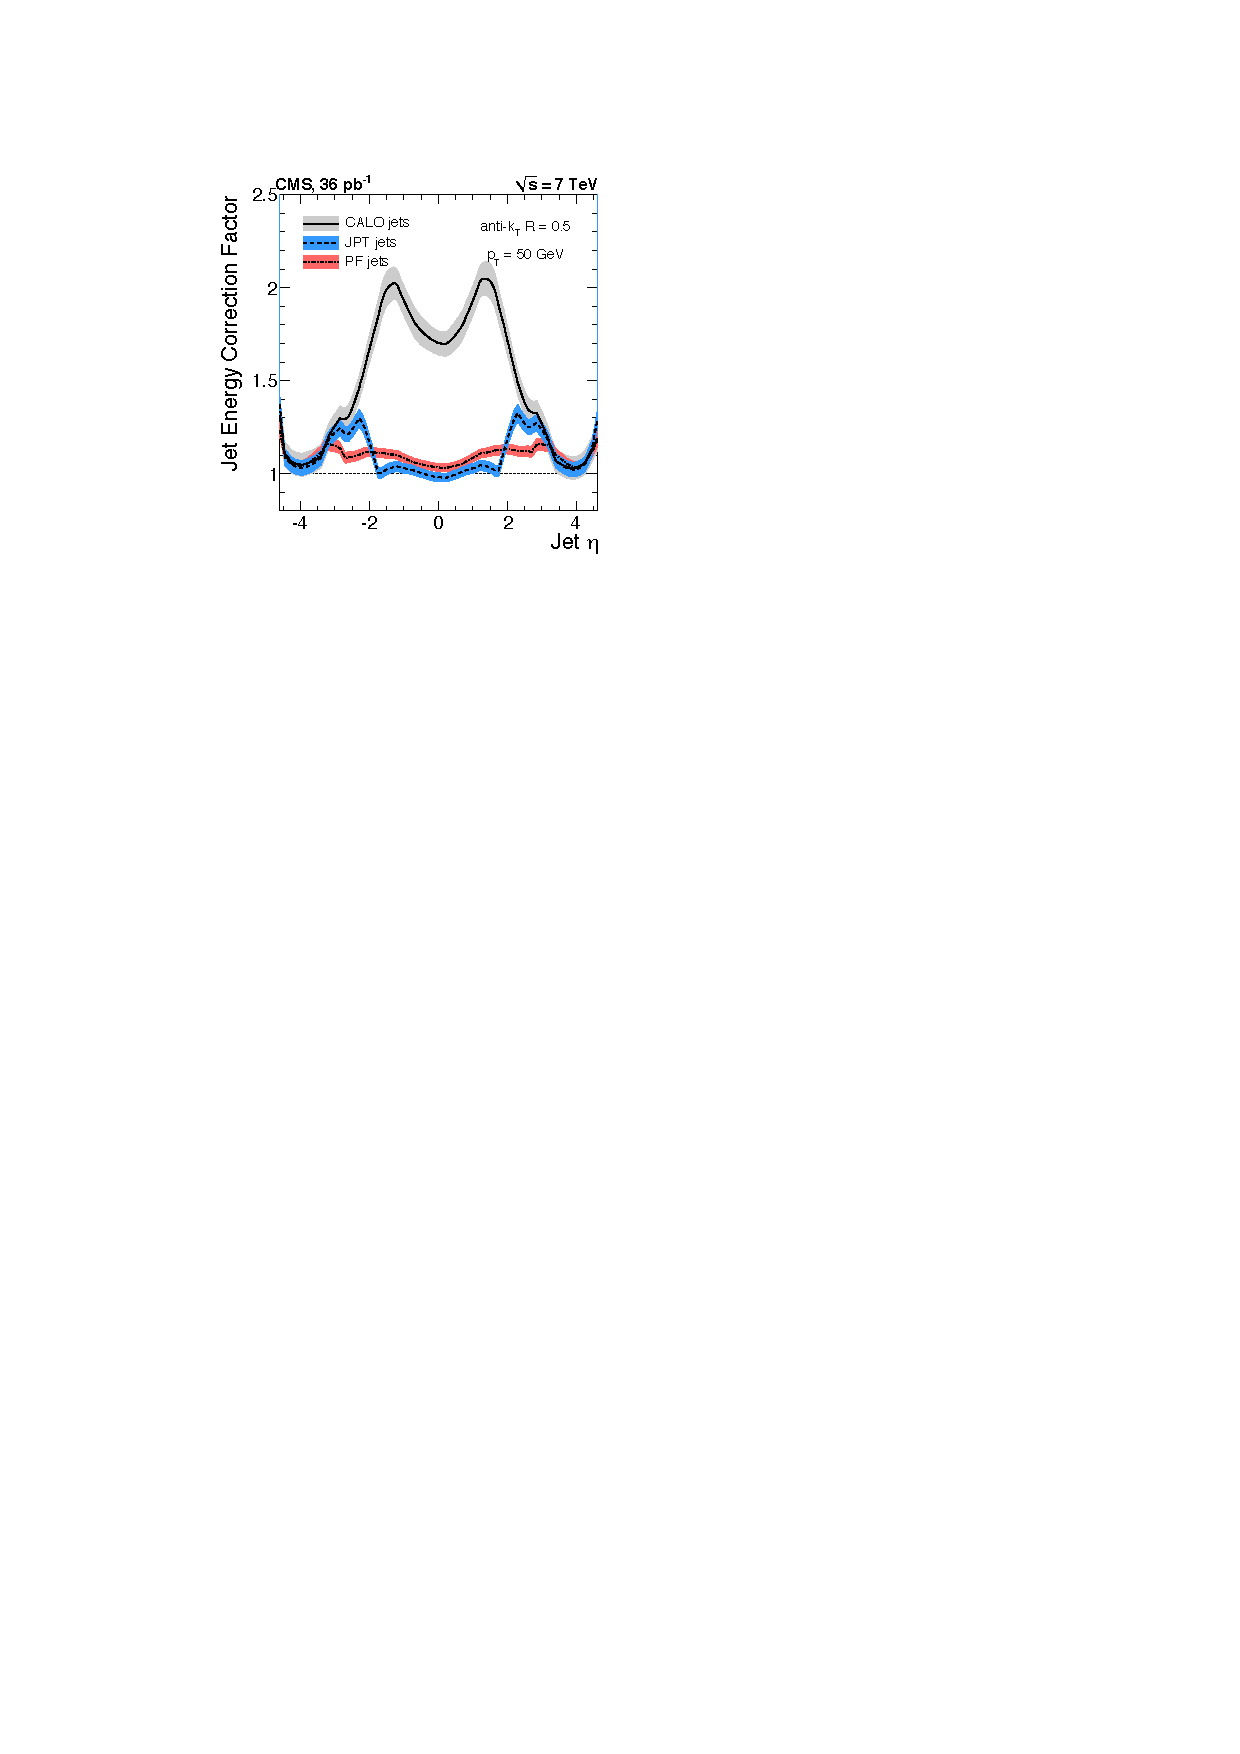
\includegraphics[width=0.5\textwidth]
      {plots/reco/jes-total-pt50.pdf}}
\subfloat[]{
    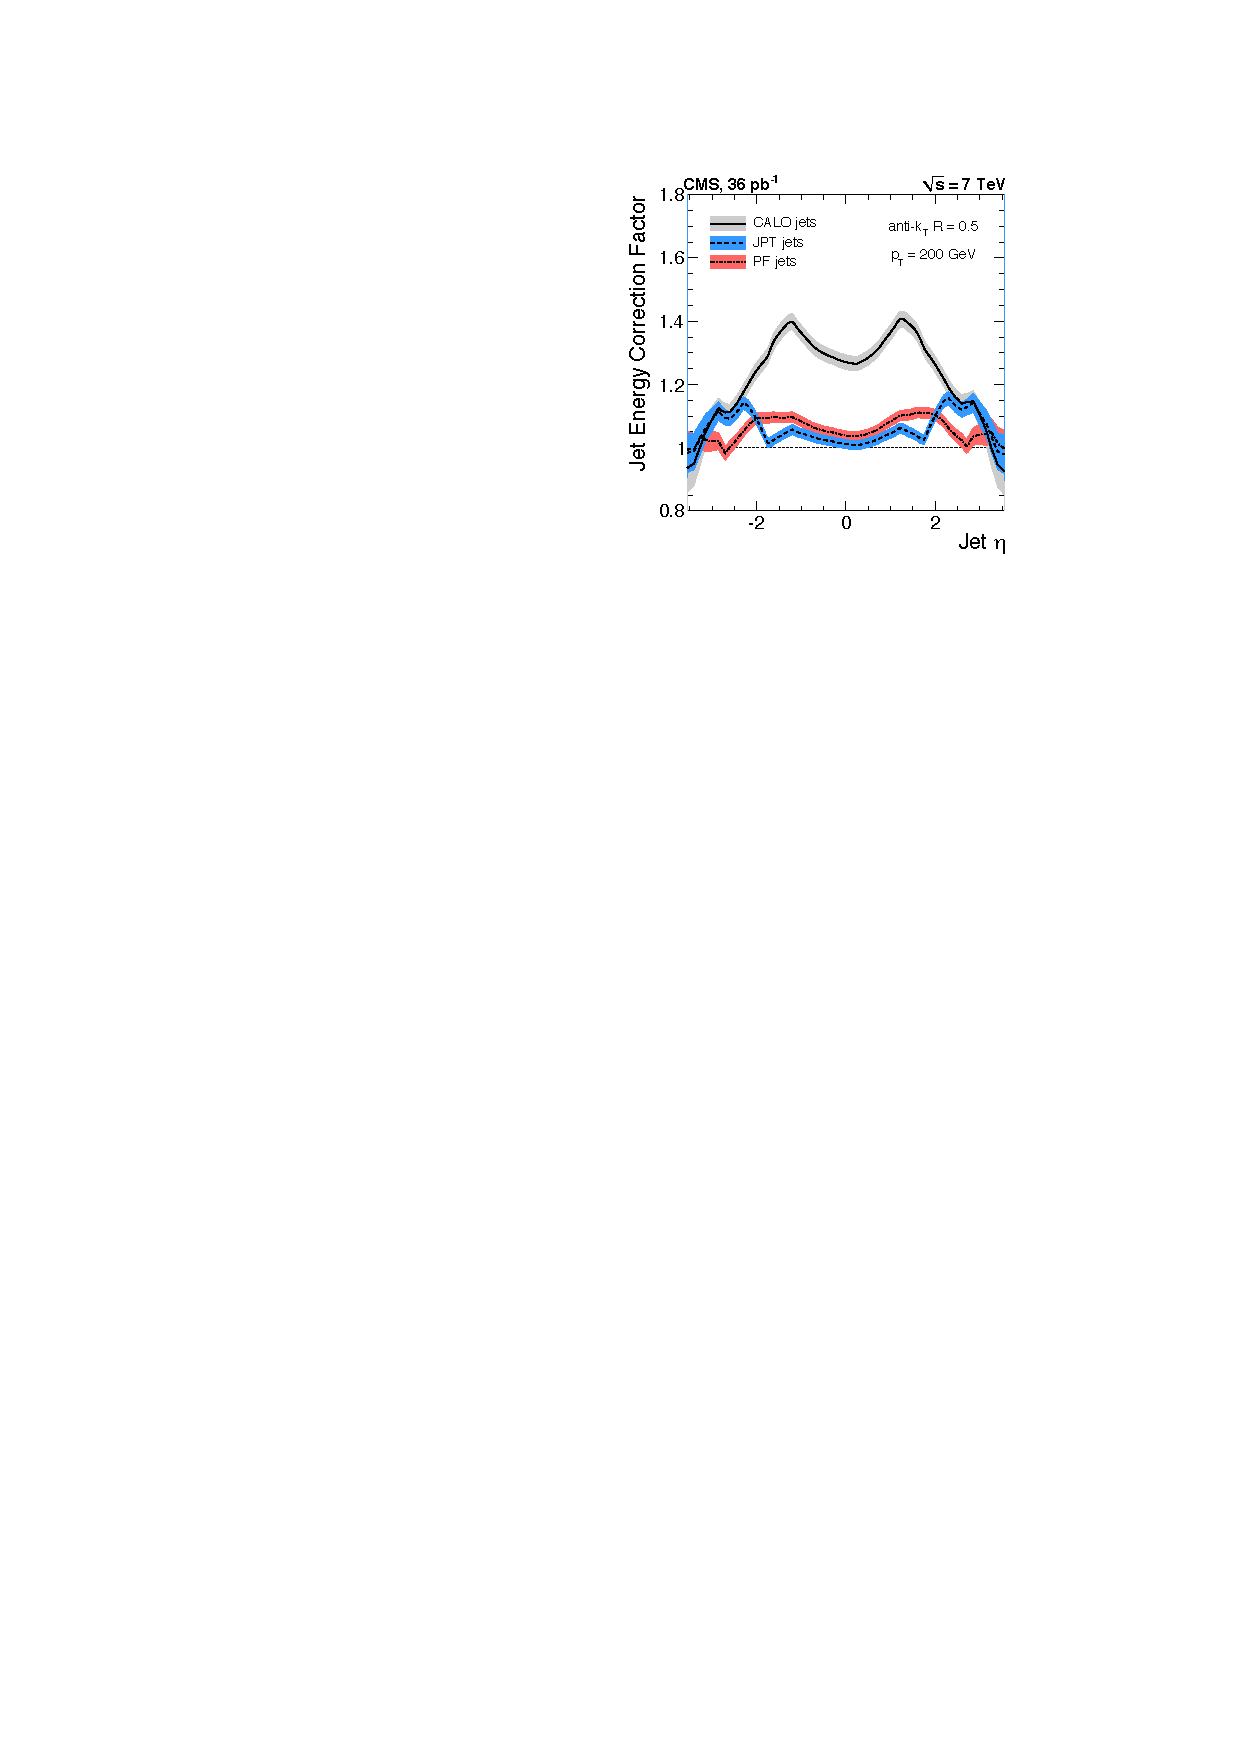
\includegraphics[width=0.5\textwidth] 
      {plots/reco/jes-total-pt200.pdf}} 

\end{center}
\caption[Total jet energy scale correction factor and corresponding uncertainty
as a function of jet $\eta$.]{
Total jet energy scale correction factor and corresponding uncertainty
as a function of jet $\eta$. Shown for jets with $\pt=50\,\GeV$ (a) and
$\pt=200\,\GeV$ (b) \cite{CMS-JME-10-011}. The correction factor is shown for
three different types of jets; only \ac{PF} jets are used in the $\HToTauTau$
analysis. For \ac{PF} jets the total uncertainty varies between $3$ and $5\%$
depending on $\pt$ and $\eta$.     
}
\label{fig:jesuncert}
\end{figure}

\subsection{B-tagged jets}
\label{sec:btag}

The identification of jets which originate from b-quarks is important in
studying many
\ac{SM} and \ac{BSM} processes. The decays of b-quarks
are suppressed by small CKM matrix elements~\cite{PDG}, giving b-flavoured hadrons relatively
long lifetimes. Such hadrons are also relatively heavy due to the large mass of
the b-quark, and as such the decay products typically have large momenta
perpendicular to the b-hadron momentum direction. Both of these features are
exploited in identification of b-tagged jets.

In the $\PH \to \Pgt\Pgt$ analysis, jets originating from b-quark
hadronisation are identified using the \ac{CSV} b-tagging
algorithm~\cite{bjets}. The long lifetime of the b-hadrons results in a
secondary decay vertex which can be reconstructed. In the \ac{CSV} algorithm, a
jet is considered b-tagged if it has $\pT>20\,\GeV$, $|\eta|<2.4$ and a
\ac{CSV} discriminator output greater than a loose, medium or tight working
point, chosen to give different levels of ID efficiency and mis-tag rates. The
inputs to the calculation of the \ac{CSV} discriminator include secondary
vertex information and the track-based lifetime information. Two likelihoods are
built from these variables, one to discriminate between b and c jets and one to
discriminate between b and light jets. 

In the $\PH\to\Pgt\Pgt$ analysis, the medium working point of the \ac{CSV}
discriminator is used to identify b-jets, corresponding to a discriminator
output greater than 0.679. The distribution of the \ac{CSV} discriminator 
can be seen in figure \ref{fig:csv}. The medium working point corresponds to a
b-tag efficiency of $\approx 85\%$ and a light jet mis-tag rate of $\approx 1\%$. 

\begin{figure}
\begin{center}
    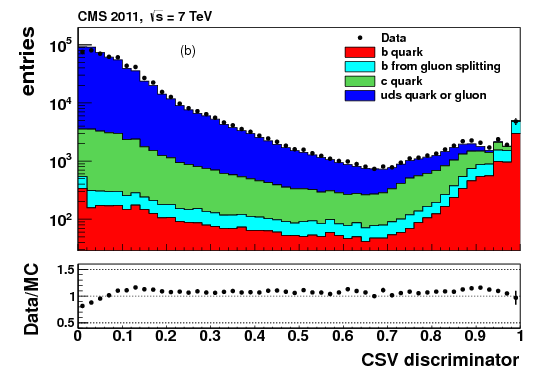
\includegraphics[width=0.6\textwidth]
      {plots/reco/csv.png}
\end{center}
\caption[The distribution of the CSV discriminator used to identify b-jets.]{
The distribution of the \ac{CSV} discriminator used to identify b-jets. The
\ac{CSV} distribution in different types of jets is highlighted \cite{bjets}.     
}
\label{fig:csv}
\end{figure}


\section{Missing energy}
\label{sec:met}

Neutrinos and any hypothetical weakly interacting stable particles do not
interact with the CMS detector. Their production is inferred from the resulting
imbalance in $\ET$ in a given event, of which the hermeticity of the CMS detector
allows measurement to a high degree of accuracy. This is crucial not only in
many searches for new physics involving such hypothetical particles, but also for
\ac{SM} processes involving neutrinos. In particular for the $\PH \to \Pgt\Pgt$
analysis accurate measurement of the $\MET$ is essential in order to reconstruct the
candidate taus after they decay via the weak interaction.

The \ac{PF} algorithm allows the calculation of $\MET$ as the opposite of the vectorial sum
of the transverse momenta of all \ac{PF} particles. 
The performance of the \ac{PF} $\MET$ response differs in data and
\ac{MC}, and a correction is derived from an independent $\PZ\to\Pmu\Pmu$ sample which
should not contain any real $\MET$ from neutrinos. The longitudinal and transverse component of
the $\pt$ response and the resolution of the $\PZ$ boson recoil is parametrised
as a function of $\pt$ and jet multiplicity. This parameterisation is then
applied to all simulated events as a function of the $\pt$ of the boson. Then
finally the $\MET$ is taken as the transverse energy of the opposite of the 
vectorial sum of the visible decay products and the
recoil~\cite{CMS-PAS-JME-12-002}. Figure~\ref{fig:PFMet} shows the distribution
of the \ac{PF} $\MET$ in $\PZ\to\Pgm\Pgm$ and $\gamma$+jet events in
$\sqrt{s}=8\,\TeV$ data and \ac{MC}. Since neither process produces any
real $\MET$, and the energy resolution of muons and photons is good, the
resolution of the $\MET$ is limited by the resolution of hadronic activity in
the event.  

\begin{figure}
\begin{center}
\subfloat[]{
    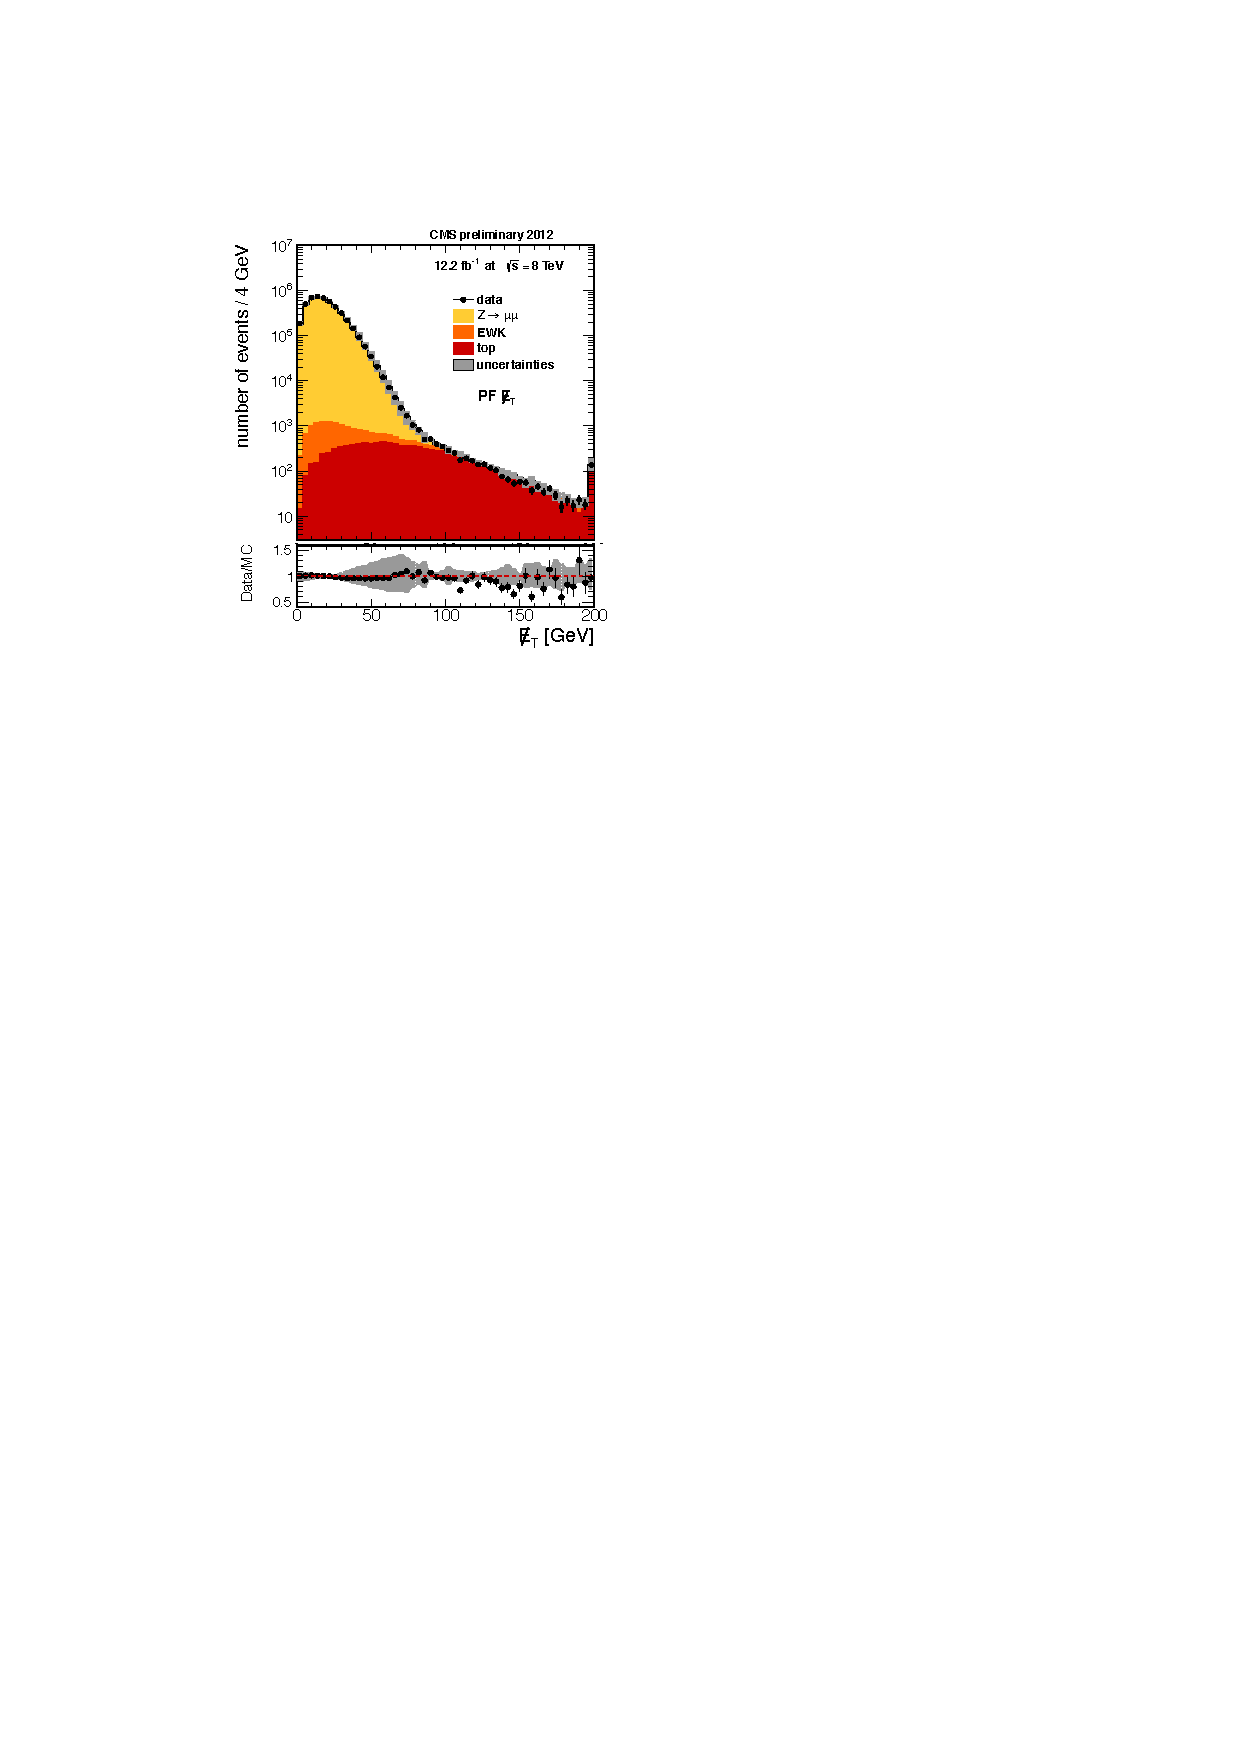
\includegraphics[width=0.5\textwidth]
      {plots/reco/PFmet_zmm.pdf}}
\subfloat[]{
    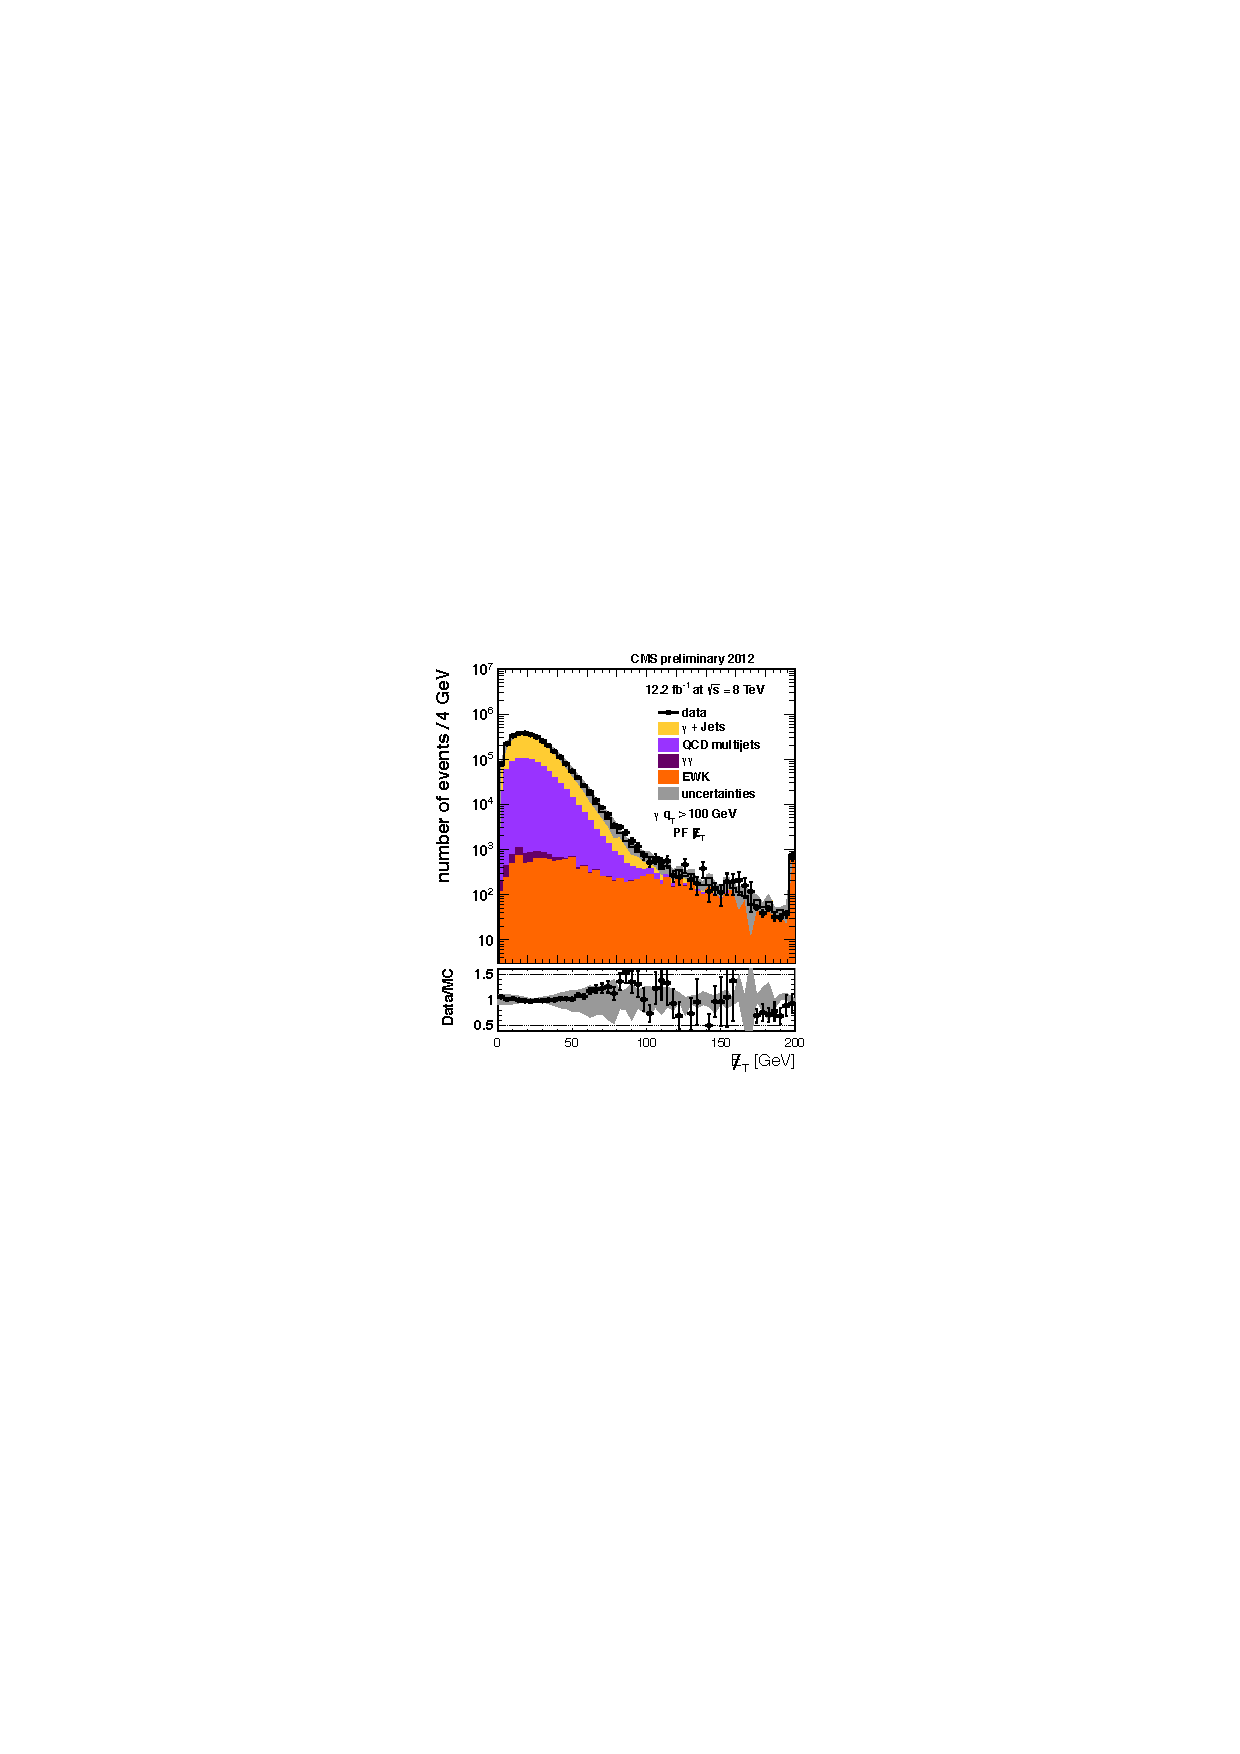
\includegraphics[width=0.5\textwidth] 
      {plots/reco/PFmet_gamma.pdf}} 
\end{center}
\caption[Distributions of PF $\MET$ in $\PZ\to\mu\mu$ and $\gamma$+jet events.]
{Distributions of \ac{PF} $\MET$ in $\PZ\to\mu\mu$ and $\gamma$+jet events for
$8\,\TeV$ data and \ac{MC}~\cite{CMS-PAS-JME-12-002}.
}
\label{fig:PFMet}
\end{figure}

The resolution of the $\MET$ can be degraded by a number of factors. These include minimum energy thresholds
in the calorimeters, non-instrumented detector regions and multiple \ac{PU}
interactions. To reduce the dependence of resolution on \ac{PU}, the $\PH\to\Pgt\Pgt$
analysis uses MVA $\MET$~\cite{CMS-PAS-JME-12-002}, 
which uses a \ac{BDT} regression multivariate analysis
including the \ac{PF} $\MET$ as one input. Other inputs are versions of the
$\MET$ calculated using the following combinations of \ac{PF} particles: 
\begin{itemize}
\item charged hadrons from the primary vertex;
\item charged hadrons from the primary vertex and neutral particles in jets
passing the pileup jet ID;
\item charged hadrons from pileup vertices and neutral particles in jets failing
the pileup jet ID;
\item charged hadrons from the primary vertex and all neutral particles in the
event, to which is added the vectorial sum of the transverse momenta of neutral
particles within jets failing the pileup jet identification.
\end{itemize}

For each type of $\MET$ the recoil is calculated as:
\begin{equation}
\vec{u} = \vecMET \cdot \hat{\phi} - \sum_{i}{\vec{\pt}^{\text{lep}}} ,
\label{eq:recoil}
\end{equation}

where $\hat{\phi}$ is the direction of the $\vecMET$ in the transverse plane and
$\vec{\pt}^{\text{lep}}$ is the $\pt$ vector of the leptons originating from the
hard interaction. The \ac{BDT} produces a correction to both the angle and the
magnitude of the \ac{PF} recoil. The final computed recoil is added to the
vector sum of leptons as in equation \ref{eq:recoil} and the resulting corrected
$\MET$ is then taken. As in the case of the \ac{PF} $\MET$, a correction is
applied for measured differences in $\MET$ response in data and \ac{MC} using
recoil corrections.

The MVA $\MET$ has a resolution which is much less
dependent on pileup, as can be seen in figure~\ref{fig:mvamet}.

\begin{figure}
\begin{center}
\subfloat[]{
    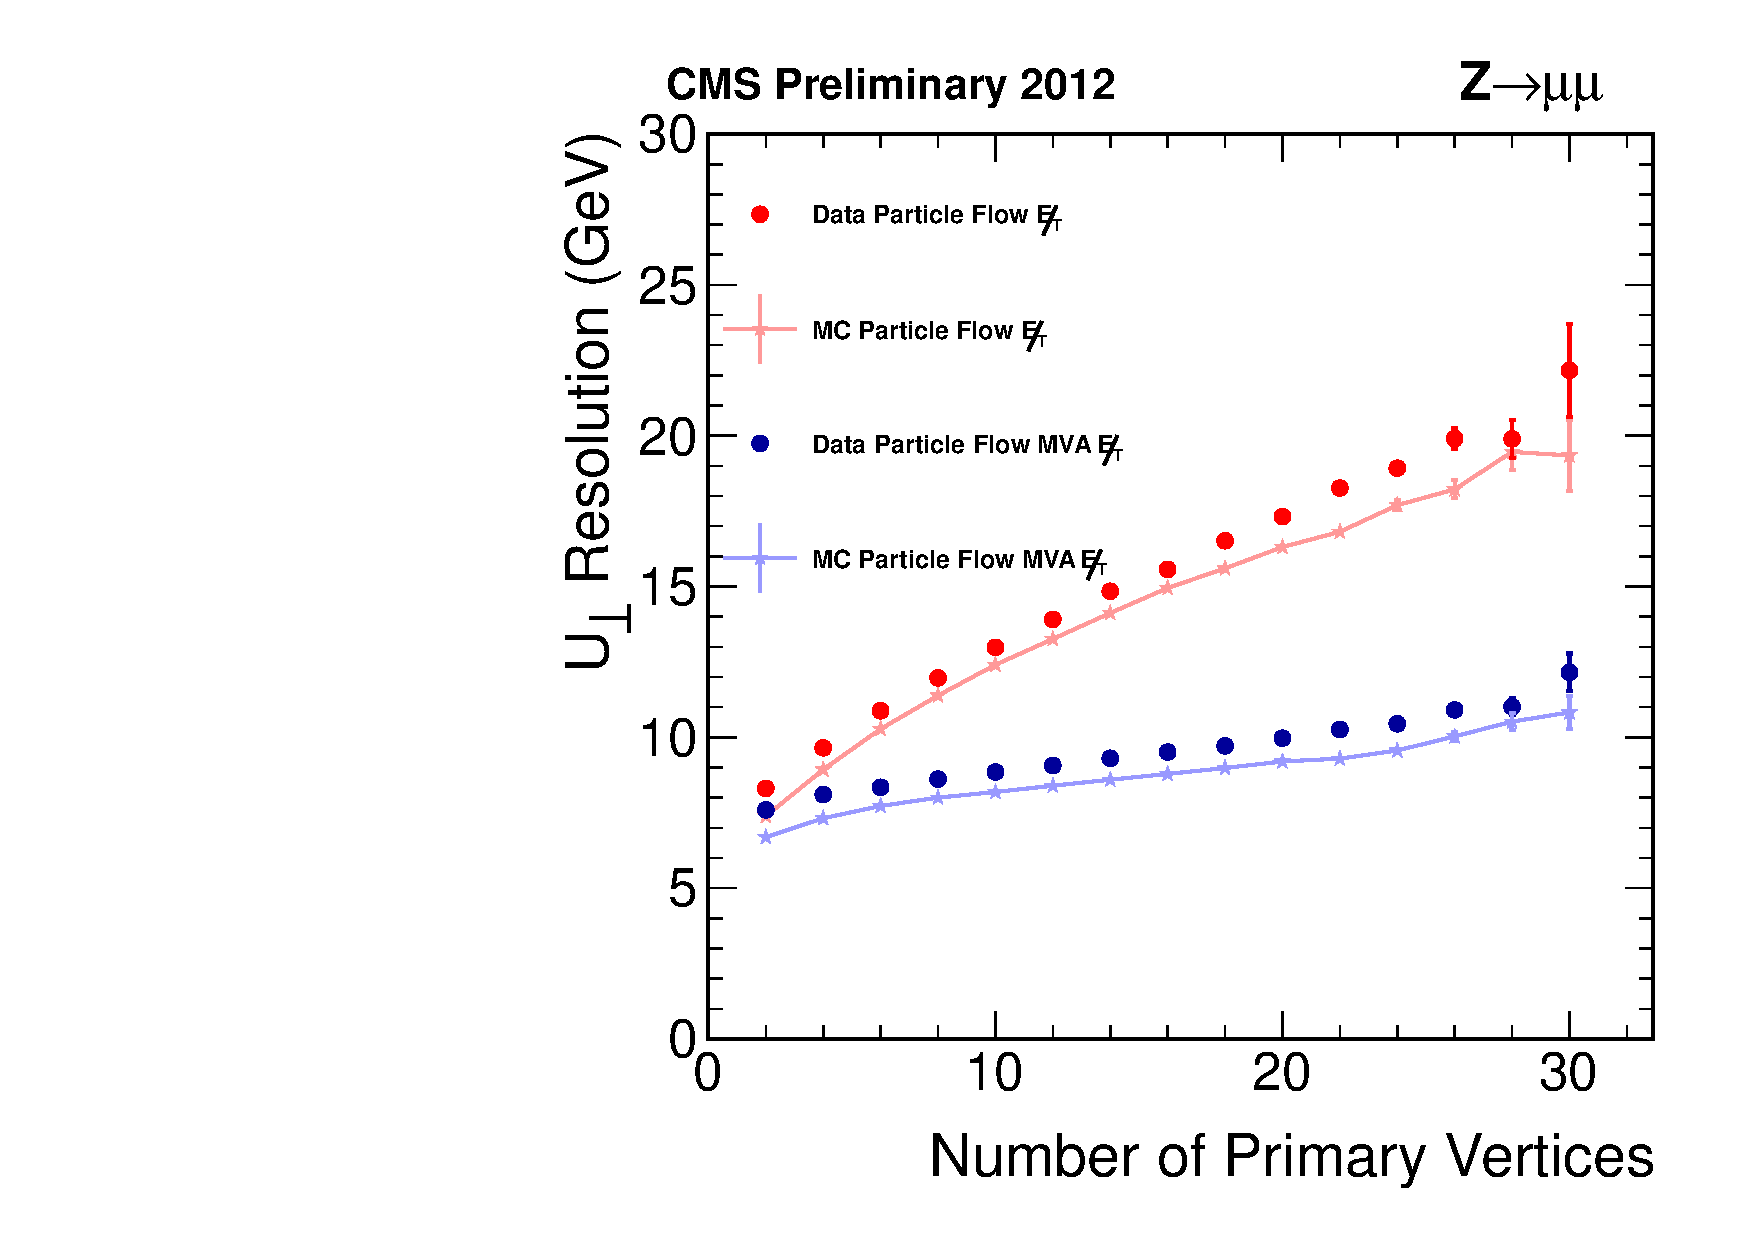
\includegraphics[width=0.5\textwidth]
      {plots/reco/U1Res.pdf}}
\subfloat[]{
    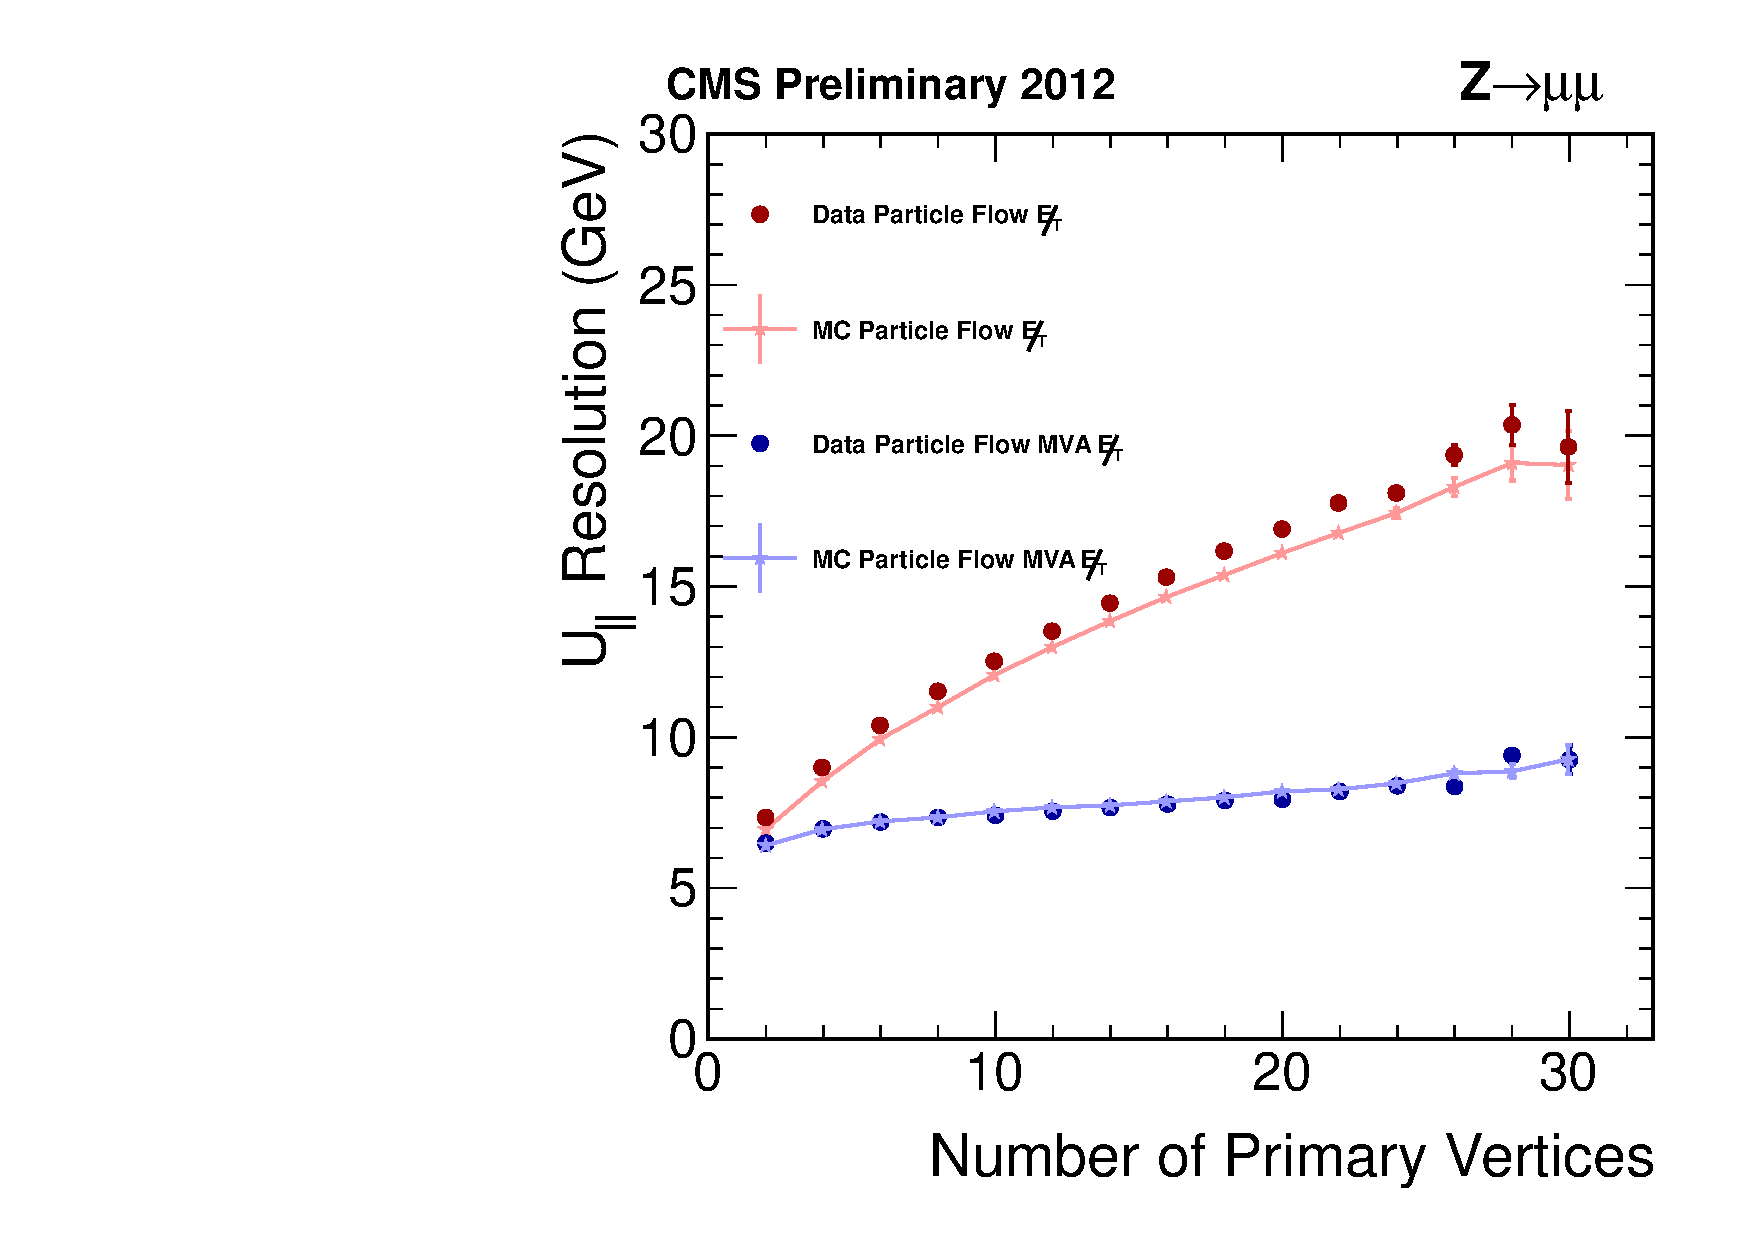
\includegraphics[width=0.5\textwidth] 
      {plots/reco/U2Res.pdf}} 
\end{center}
\caption[The dependence of the resolution of the hadronic
recoil response on the number of primary vertices in the event for PF
$\MET$ and MVA $\MET$.]
{The dependence of the resolution of the hadronic
recoil response on the number of primary vertices in the event for \ac{PF}
$\MET$ and MVA $\MET$~\cite{CMS-PAS-JME-12-002}.
}
\label{fig:mvamet}
\end{figure}

\section{Hadronic taus}
\label{sec:taus}

Taus decay via the weak force. Approximately $35\%$ of the time, they decay into a final state consisting of a tau
neutrino, an electron/muon and the associated electron/muon neutrino. 
This section describes the identification of taus for the other $\sim65\%$ of the time,
when they decay into a tau neutrino plus quarks yielding a hadronic tau, $\Pgth$. The different
possibilities for hadronic tau decays are listed in table~\ref{tab:hadronictaus}.

\begin{table}[bth]
\begin{tabular}{|c|c|c|}
\hline
Decay Mode & Intermediate Resonance & Branching Fraction [\%] \\
\hline
\hline
$\Pgtpm\to\Pgppm\Pgpz\Pgngt$ & $\Pgr$(770) & 25.5 \\
\hline
$\Pgtpm\to\Pgppm\Pgngt$ & -  & 10.8 \\
\hline
$\Pgtpm\to\Pgppm\Pgpz\Pgpz\Pgngt$ & $\text{a}_{1}$(1260) & 9.3 \\
\hline
$\Pgtpm\to\Pgppm\Pgpmp\Pgppm\Pgngt$ & $\text{a}_{1}$(1260) & 9.3 \\
\hline
$\Pgtpm\to\Pgppm\Pgpmp\Pgppm\Pgpz\Pgngt$ & -  & 4.6 \\
\hline
Other hadronic modes & - & 5.3 \\
\hline
\hline
Total & &  64.7 \\
\hline
\end{tabular}
\caption[List of the possible hadronic tau decay modes.]{List of the possible hadronic tau decay modes. The branching ratios for
each is given, and where the decay proceeds via an intermediate resonance this
is given along with its mass in $\MeV$ \cite{PDG}.}
\label{tab:hadronictaus}
\end{table}

The largest fraction of hadronic decays proceed via the $\Pgr$(770) resonance
resulting in one charged and one neutral pion. Other common modes produce
different numbers of neutral or charged pions. Decays with more than 3 charged
pions are included in the other hadronic modes listed in the table and are
relatively rare. The knowledge of the number of pions in the final state is used in the
identification of hadronic taus.

Hadronic taus are a collection of hadronic particles and as such the first level
of identification is similar to jet ID. 
Since the decay products come directly from the tau they are constrained by the
tau mass. This results in a highly collimated hadronic system compared with the
typical jet. This provides differentiation between hadronic taus and
quark and gluon jets. This property is utilised in the tau isolation.

\subsection{Hadron plus strips algorithm}
\label{sec:hps}

For the $\PH \to \Pgt\Pgt$ analysis, the \ac{HPS} algorithm is used to identify
hadronic taus \cite{CMS-PAS-TAU-11-001}. The \ac{HPS} algorithm makes use of \ac{PF} candidates to reconstruct the
charged pions and the photons resulting from the decays of the neutral pions. In
addition, the masses of the intermediate resonances listed in table \ref{tab:hadronictaus} can be
applied. In this algorithm only the visible products of the taus are considered
- the tau neutrino forms part of the missing energy.

The algorithm is seeded by a \ac{PF} jet, which is reconstructed as described in
section \ref{sec:jetID} with distance parameter $R=0.5$. The photons from the neutral pion decay have a high
probability to convert to electron-positron pairs within the tracker, resulting
in an EM shower spread in the $\phi$ direction. These candidates are clustered
using strips with size $\Delta\eta = 0.05$ and $\Delta\phi = 0.2$ initially
centred on the most energetic EM candidate in the \ac{PF} jet. Strips with
$\pt>1\,\GeV$ are considered. The extracted mass of the
strip is required to be consistent with the mass of the neutral pion, and hence
between 50 and $200\,\MeV$. The strips are then combined with the charged hadrons
from \ac{PF} to give four different cases:

\begin{itemize}
\item Single charged hadron or ``prong'', no strips: corresponds to $\Pgtpm\to\Pgppm\Pgngt$,
with some contribution from $\Pgtpm\to\Pgppm\Pgngt\Pgpz$ in the case that the
neutral pion is not energetic enough to be detected.
\item Single charged hadron or prong, one strip: this selects decays to the intermediate
resonance of $\Pgr$(770), $\Pgtpm\to\Pgrpm\Pgngt\to\Pgppm\Pgpz\Pgngt$. In this
case the combined system must have invariant mass consistent with the
$\Pgr$(770).
%or $\text{a}_{1}$(1260), so between 300 and 1300 $\MeV$. %check - is the lower
%bound 300 or 400? 
\item Single charged hadron or prong, two strips: corresponds to
$\Pgtpm\to\Pgppm\Pgpz\Pgpz\Pgngt$. Here, consistency of the mass with the
$\text{a}_{1}$(1260) resonance is required. 
\item Three charged hadrons or prongs: these correspond to
$\Pgtpm\to\Pgppm\Pgpmp\Pgppm\Pgpz\Pgngt$ or $\Pgtpm\to\Pgppm\Pgpmp\Pgppm\Pgngt$. 
In this case, the tracks are required
to come from the same vertex, with a minimum impact parameter in the transverse
plane of $2\,\mm$. The three candidates must also have total charge of 1, and a
mass consistent with $\text{a}_{1}$(1260). 
\end{itemize}

In all of the above cases, the charged hadrons and strips must be contained
within a cone defined by $\Delta R=2.8\,\GeV/\pt^{\Pgth}$, where
$\pt^{\Pgth}$ is the $\pt$ of the hadronic tau candidate, for taus with $28 <
\pt^{\Pgth} < 56\,\GeV$. For taus with $\pt^{\Pgth} < 28\,\GeV$ the cone is
is fixed at 0.1 and for taus with $\pt^{\Pgth} > 56\,\GeV$ at 0.05. 
Figure \ref{fig:taudecaymode} illustrates the number of events reconstructed in
each of the tau decay modes in the backgrounds to the $\PH \to \Pgt\Pgt$ analysis.

\begin{figure}
\begin{center}
    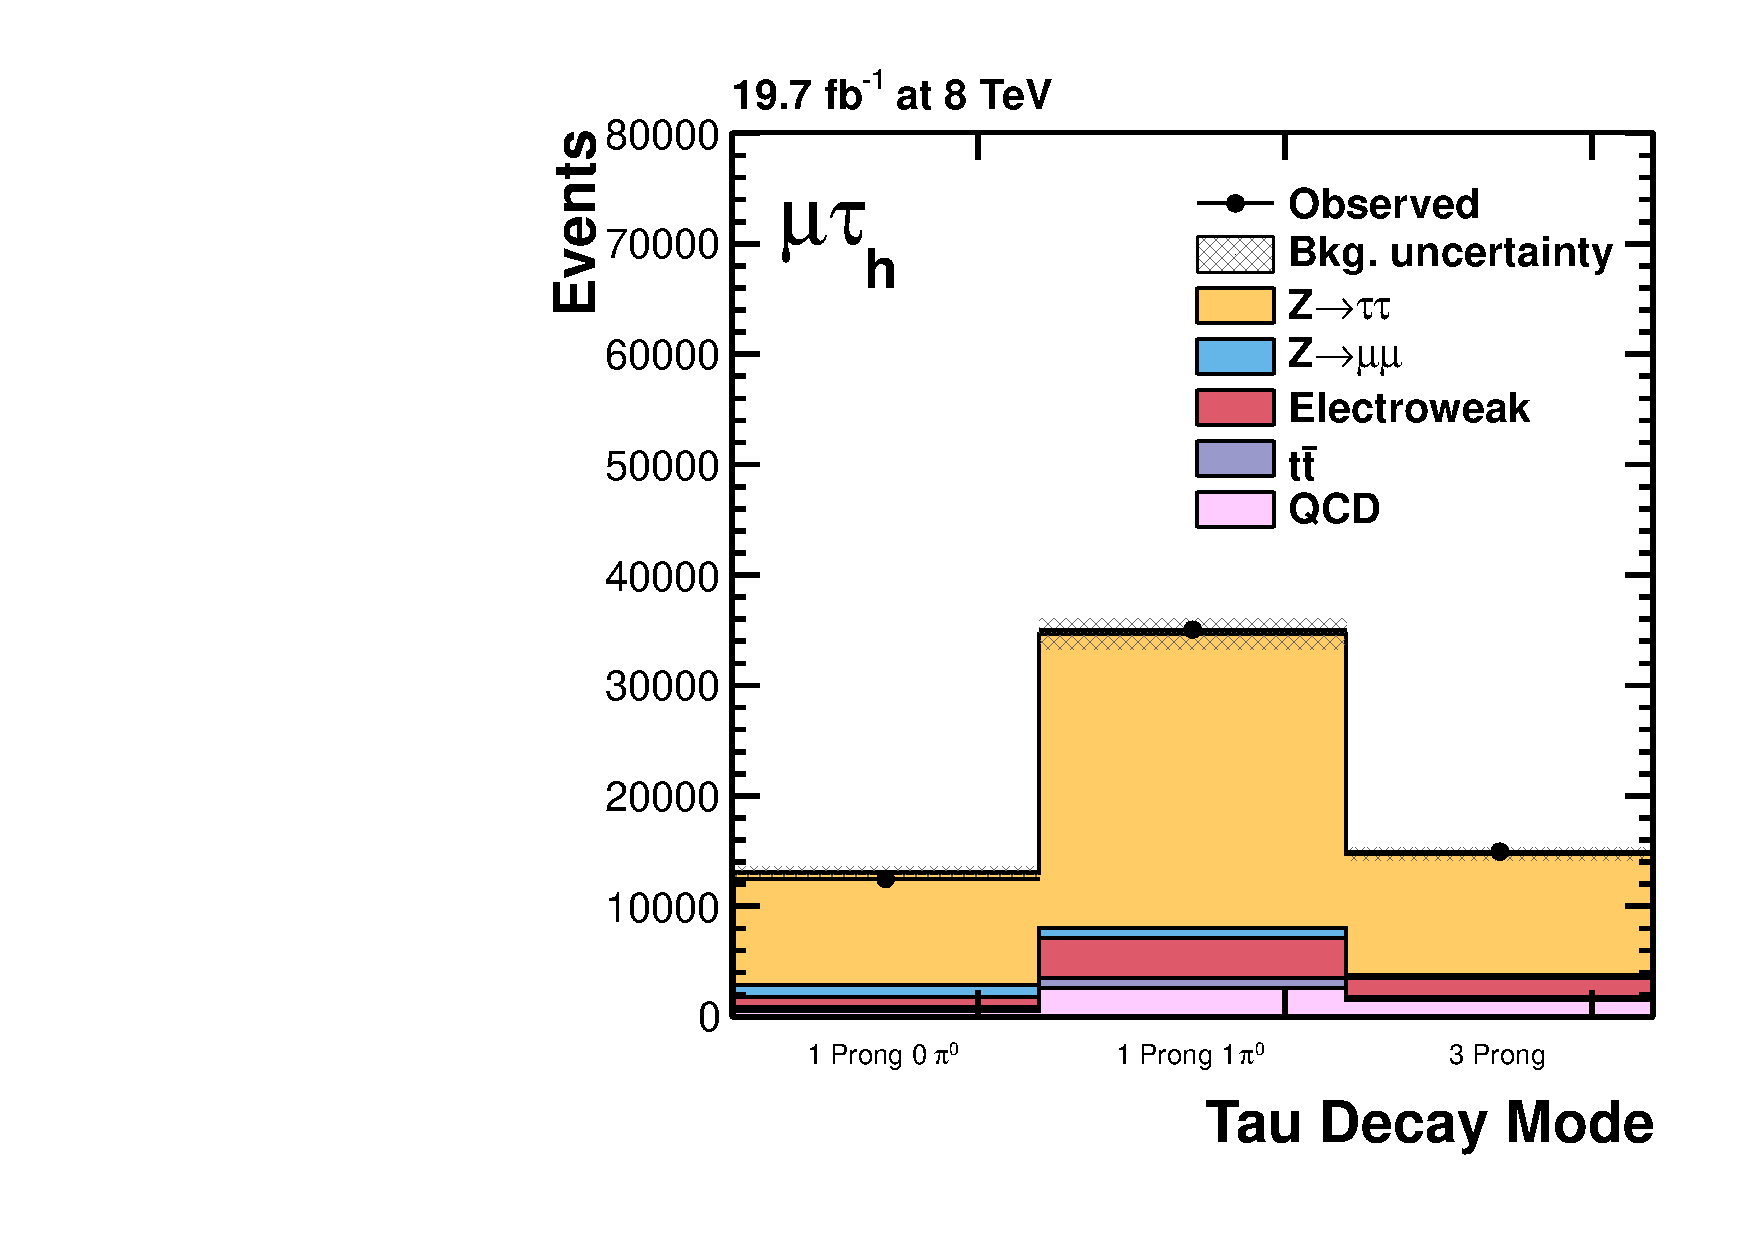
\includegraphics[width=0.5\textwidth]
      {plots/reco/tau_decay_mode_inclusive_mt_2012.pdf}
\end{center}
\caption[Figure illustrating the fraction of events in each tau decay mode in the
$\mutau$ channel of the $\PH\to\Pgt\Pgt$ analysis.]
{Figure illustrating the fraction of events in each tau decay mode in the
$\mutau$ channel of the $\PH\to\Pgt\Pgt$ analysis. The term ``prong'' refers to a
charged hadron. The ``1 prong 1 \Pgpz'' bin contains both single charged hadron
with one strip and single charged hadron with two strips, defined in the text.
}
\label{fig:taudecaymode}
\end{figure}

\subsection{Isolation}
\label{sec:tauisolation}

A measure of the isolation of the hadronic tau candidate is used to exploit the
collimated nature of the $\tau$-jets to reduce the background from quark and gluon
jets. The isolation is computed in the same way as in
equation~\ref{eq:leptonisolation} for
electrons and muons. The isolation variable is constructed from 
the sum of the $\pt$ of the
hadronic and photon \ac{PF} candidates with $\pt > 0.5\,\GeV$ within a cone centred on 
the $\Pgth$ with size $\Delta R = 0.5$. The charged hadrons in the sum are
required to have $\Delta z < 2\,\mm$ with respect to the production vertex of the
$\Pgth$. The charged hadrons associated with other vertices (i.e. with
$\Delta z > 2\mm$) are used to estimate and subtract the contribution to the isolation 
from photons produced in \ac{PU} interactions, using a cone of size $\Delta R = 0.8$. 
All constituent particles of the $\Pgth$ candidate are excluded from the
calculation. Different working points of the isolation are chosen to correspond to 
loose, medium and tight working points of tau isolation.   

\subsection{Electron and muon rejection}
\label{sec:tauleptonrejection}

An electron can be misidentified as an hadronic tau with one charged hadron when
it has an isolated energy deposit in the calorimeters. Electrons can also be
reconstructed as hadronic taus in the one charged hadron plus strips modes when 
they emit photons via bremsstrahlung. A \ac{BDT} is trained to reduce
misidentified electrons, using many of the same variables exploited in electron
ID described in section \ref{sec:electrons}. The $\PH\to\Pgt\Pgt$ analysis makes 
use of this discriminator in a tight working point in all final states except
for $\etau$, which reduces the rate 
of misidentified electrons to around $3\%$ with an efficiency for real taus of
around $90\%$. 

The probability of a muon to produce a fake hadronic tau is much lower. Such
events are suppressed by requiring that the track of the leading charged hadron
constituent in the hadronic tau is not also reconstructed as a tracker muon.
Loose, medium and tight working points are available for this discriminator
also, depending on how strict the criteria are in determining whether or not
this track matches a signal in the muon systems. 

\subsection{Energy scale}
\label{sec:taues}

As with jets, corrections are needed to ensure that the energy scale
of hadronic taus in \ac{MC} matches that in data. The inclusive selection in the
$\PH \to \Pgt\Pgt$ analysis yields a large number of $\ZToTauTau$ events. The
distribution of the tau mass can be fit separately for each decay mode, allowing
the $\ZToTauTau$ events to constrain the tau energy scale. This is done
separately for different ranges of tau $\pt$, allowing the tau energy scale to
float freely in each fit. The result is a set of $\pt$ and decay mode dependent
corrections which are applied to \ac{MC}. Figure \ref{fig:taumass} shows the
resulting tau mass distribution for the $\mutau$ channel of the $\PH\to\Pgt\Pgt$
analysis. The resulting uncertainty on the tau energy scale is found to be $3\%$.

\begin{figure}[htb]
\begin{center}
    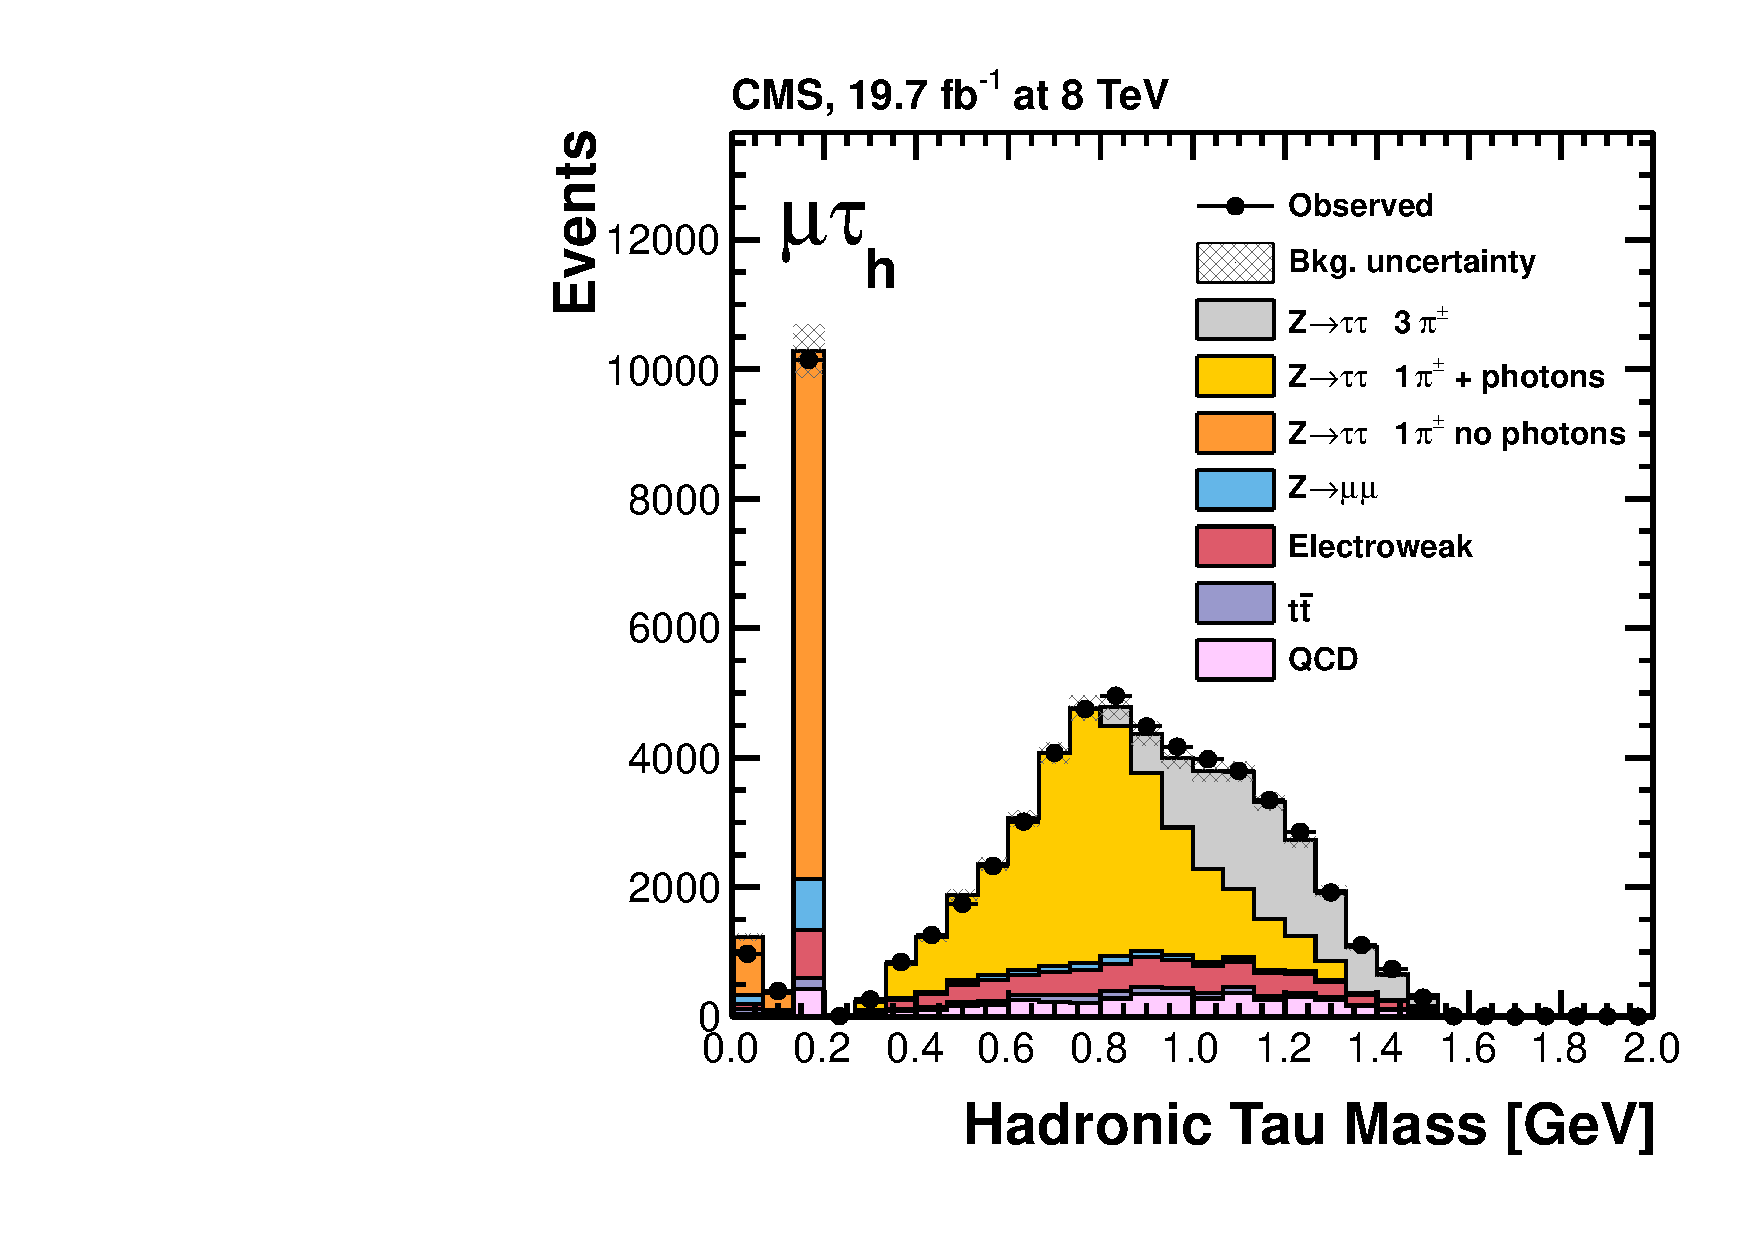
\includegraphics[width=0.5\textwidth]
      {plots/reco/m_2_tau_modes_mt_2012.pdf}
\end{center}
\caption[The invariant mass of the hadronic tau in $\mutau$ channel events of
the $\PH\to\Pgt\Pgt$ analysis.]{The invariant mass of the hadronic tau in $\mutau$ channel events of
the $\PH\to\Pgt\Pgt$ analysis. The $\PZ\to\Pgt\Pgt$ component is separated into the
different decay modes of the tau. Decays with only one charged hadron are
typically assigned the pion mass by the \ac{PF} algorithm, except for a small
fraction which are assigned the muon or electron mass and are found in the first
two bins. The contribution from candidates with one charged hadron and photons
peaks near the mass of the intermediate $\rho(770)$ meson, and from those with
three charged hadrons peaks near the mass of the $\text{a}_{1}(1260)$ meson.}
\label{fig:taumass}
\end{figure}

In subsequent chapters, the term ``tau'' is often used to mean ``hadronic tau'',
where the meaning is clear from the context.

\section{Di-tau mass reconstruction in $\PH \to \Pgt\Pgt$}
\label{sec:svfit}

In $\PH \to \Pgt\Pgt$ events, the mass of the Higgs boson is reconstructed by
the di-tau mass, $m_{\Pgt\Pgt}$. This is important in distinguishing possible $\PH\to\Pgt\Pgt$
events from the irreducible $\PZ \to \Pgt\Pgt$ process, since both processes
include real taus in the final state and only differ in the invariant mass of the tau pair. 
The reconstruction of the mass of the tau pair is made less straightforward
by the fact that the taus themselves decay to both visible and invisible
products. The visible products of leptons and hadronic taus can be combined to
reconstruct a quantity referred to as visible mass, $m_{\text{vis}}$,
but greater accuracy is achieved if the full mass is reconstructed including the
invisible neutrinos. This can be achieved using a likelihood based algorithm called
SVFit~\cite{HIG-13-004}, which combines the visible decay products and the reconstructed $\MET$. A
short description of this method is given in this section. A more detailed
description can be found in \cite{HIG-13-004,Bianchini:2014vza}.

The inputs to the SVFit algorithm are the kinematics of the visible decay
products and the missing transverse energy. If all visible components of a
hadronic tau decay are treated as a single composite object, the visible part of
the decay is specified by five parameters, which are chosen to be the momentum,
polar and azimuthal angles in the lab frame, and two decay angles in the rest
frame of the tau lepton. Leptonic tau decays produce an additional neutrino, and so an additional
variable is required to describe the invisible part of the decay, 
which is chosen to be the invariant mass of the
two-neutrino system (this is zero in the case of hadronic tau decays). 
The unknown parameters are constrained by three
observables: the momentum, polar and azimuthal angles of the visible products
measured in the lab frame. Further constraints are provided by
$E_{x}^{\text{miss}}$ and $E_{y}^{\text{miss}}$, the x and y components of the
$\MET$, within the experimental resolution. This leaves either two or three 
unconstrained parameters for the hadronic or leptonic tau decay respectively. 
These are chosen to be:

\begin{itemize}
\item $x$: the fraction of the energy of the tau carried by the visible decay
products in the lab frame.
\item $\phi$: the azimuthal angle of the tau in the lab frame. 
\item $m_{\nu\nu}$: the mass of the neutrino system. This is set to zero for hadronic tau
decays which have only one neutrino.
\end{itemize}

The SVFit algorithm employs a likelihood approach, in which possible
$m_{\Pgt\Pgt}$ values are reconstructed by combining $E_{x}^{\text{miss}}$ and
$E_{y}^{\text{miss}}$ with a probability model with terms to account for the tau
decay kinematics and $\MET$ resolution. The vector $\vec{a}$ is defined to
specify the kinematics of each tau decay as $\vec{a} =
\left(x_{1},\phi_{1},m_{\nu\nu}^{1},x_{2},\phi_{2},m_{\nu\nu}^{2}\right)$, where
the labels $1$ and $2$ refer to each of the two taus. Then the
probability that the values of $\vec{x} = \left(E_{x}^{\text{miss}},
E_{y}^{\text{miss}}\right)$ are observed, given that the momenta of the visible decay products are
equal to the observed $\vec{y} = \left(p_{1}^{vis},p_{2}^{vis} \right)$,
yielding a value of $m_{\Pgt\Pgt}^{i}$, is given by: 

\begin{equation} \label{eqn:svfit-prob}
P(m_{\Pgt\Pgt}^{i}) = \int\delta\left(m_{\Pgt\Pgt}^{i} -
m_{\Pgt\Pgt}(\vec{y},\vec{a})\right)p(\vec{x},\vec{y},\vec{a})\,\text{d}\vec{a}\,
.
\end{equation}

The best estimate $m_{\Pgt\Pgt}^{i}$ for the value of $m_{\Pgt\Pgt}$ is then the value which maximises this probability. 

Likelihood functions are used to model the tau decay kinematics. These are
different for hadronic and leptonic tau decays. For hadronic tau decays, a model
based on two-body phase space is used \cite{PDG}, in which all the decay products of the
tau are grouped to be one particle:

\begin{equation}
\mathcal{L}_{\Pgt}^{\text{had}} = \frac{\text{d}\Gamma}{\text{d}x\,\text{d}\phi}
\propto \frac{1}{1 - m_{\text{vis}}^{2} / m_{\Pgt}^{2}},
\end{equation}

which is valid in the physically allowed region of $m_{\text{vis}}^{2} /
m_{\Pgt}^{2} \leq x \leq 1$. The leptonic function is derived using a matrix
element approach \cite{TauPol}:

\begin{equation}
\mathcal{L}_{\Pgt}^{\text{lep}} =
\frac{\text{d}\Gamma}{\text{d}x\,\text{d}m_{\nu\nu}\,\text{d}\phi} \propto
\frac{m_{\nu\nu}}{4m_{\Pgt}^{2}}\left[(m_{\Pgt}^{2}+2m_{\nu\nu}^{2})(m_{\Pgt}^{2}-m_{\nu\nu}^{2})\right],
\end{equation}

for which the physically allowed region constitutes $0 \leq x \leq 1$ and $0
\leq m_{\nu\nu} \leq m_{\tau}\sqrt{1-x}$. The final part of the likelihood
quantifies the compatibility of a particular tau decay hypothesis with the
reconstructed $\MET$. The resolution of the neutrino energy measurement is
modelled using a Gaussian form:

\begin{equation}
\mathcal{L}_{\nu}(E_{x}^{\text{miss}},E_{y}^{\text{miss}}) =
\frac{1}{2\pi\sqrt{|V|}}\text{exp}\left[
-\frac{1}{2}\begin{pmatrix}E_{x}^{\text{miss}}-\sum p_{x}^{\nu} \\
E_{y}^{\text{miss}}-\sum p_{y}^{\nu}\end{pmatrix}^{T} V^{-1}
\begin{pmatrix}E_{x}^{\text{miss}}-\sum p_{x}^{\nu} \\ E_{y}^{\text{miss}}-\sum
p_{y}^{\nu}\end{pmatrix}\right].
\end{equation}

In this equation $V$ is the covariance matrix which accounts for the expected
resolution of the $\MET$ reconstruction, and is determined for each event from
the MVA MET algorithm described in section \ref{sec:met}. This resolution is
typically $10$-$15\,\GeV$. 

Figure \ref{fig:svfit} shows the shape comparison between $\PH\to\Pgt\Pgt$ signal
and $\PZ \to \Pgt\Pgt$ background in the case of using the visible mass or the mass from SVFit. It can
be seen that the shape separation is greatly improved in the SVFit case.
The improvement in expected limit from using SVFit over visible mass in the $\PH
\to \Pgt\Pgt$ analysis is around 40$\%$. The use of SVFit mass in the
$\PH\to\Pgt\Pgt$ analysis is discussed further in the next chapter.

\begin{figure}[tbh]
\begin{center}
\subfloat[]{
    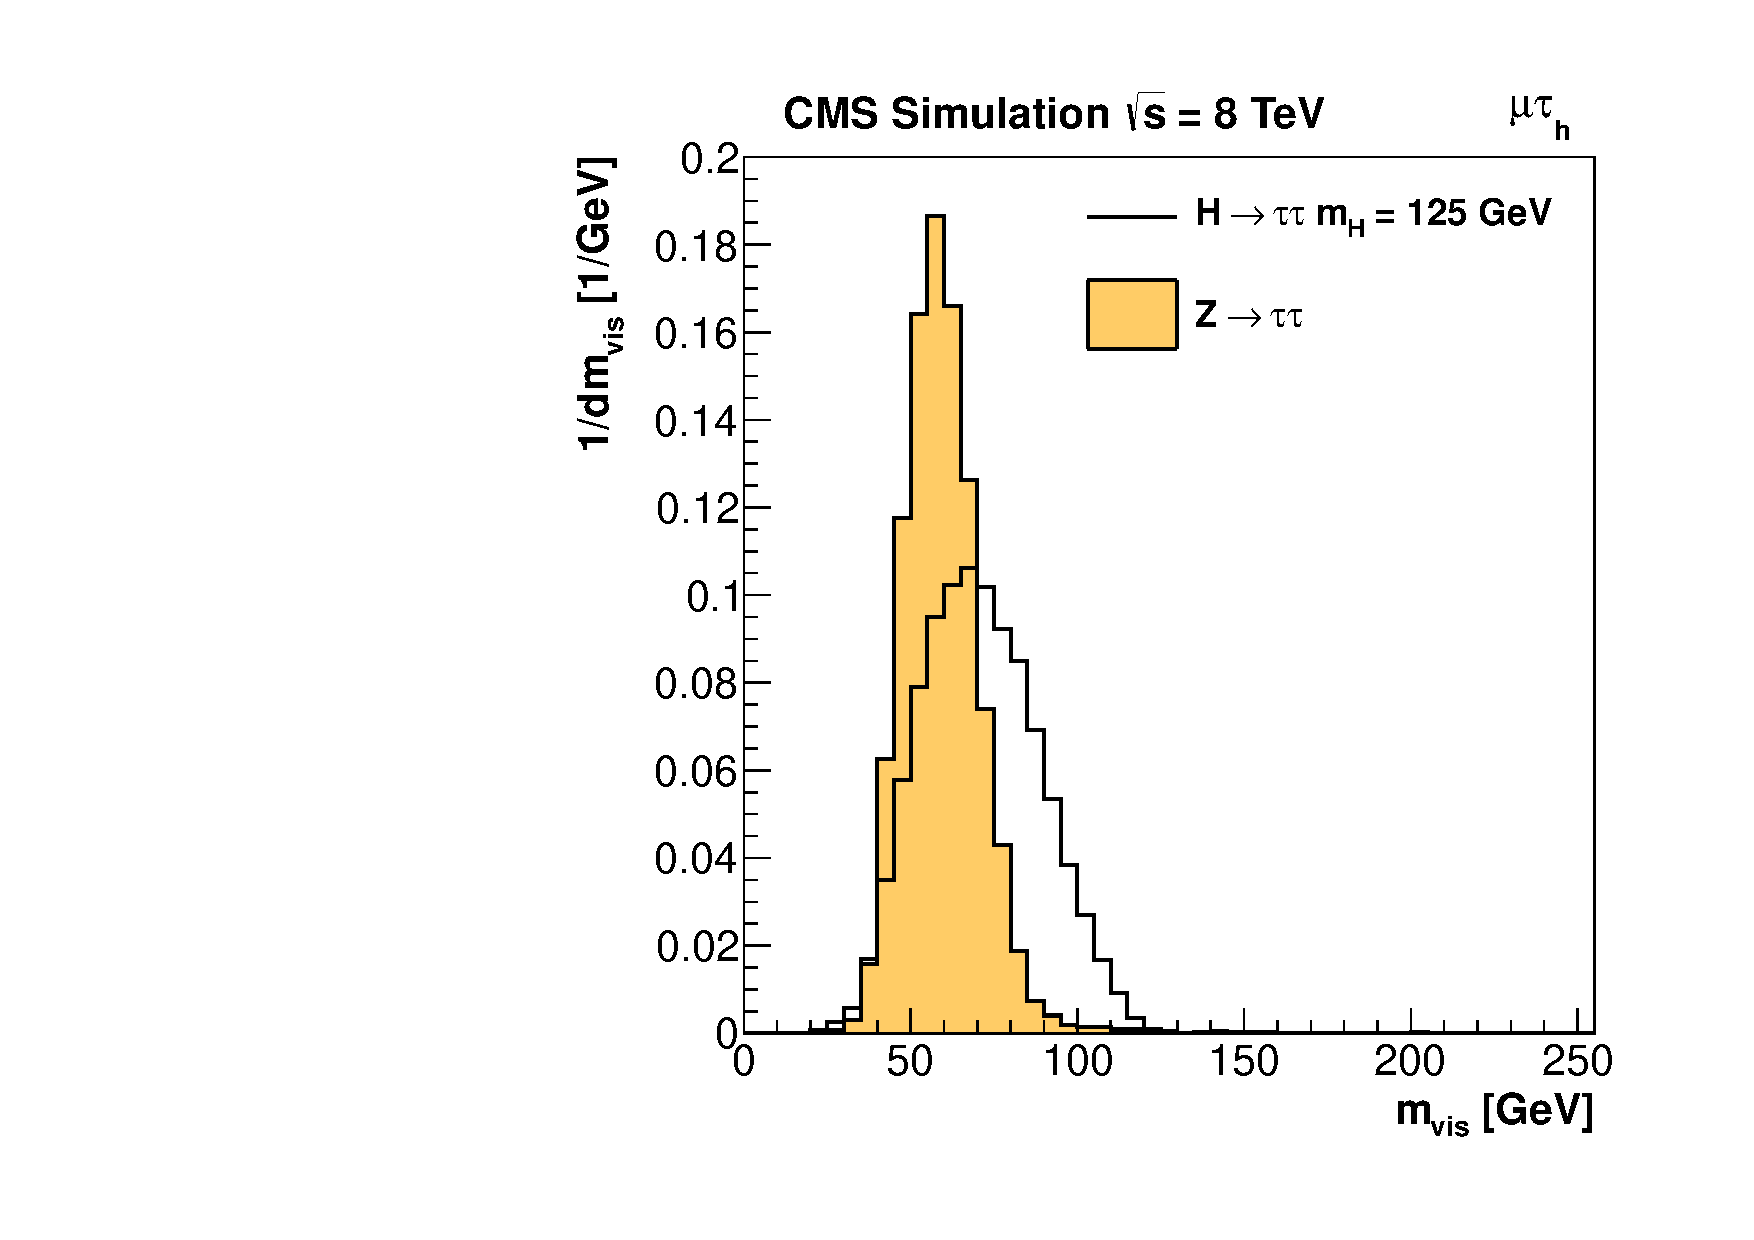
\includegraphics[width=0.5\textwidth]
      {plots/reco/svFitPerformance_forColin_visMass.pdf}}
\subfloat[]{
    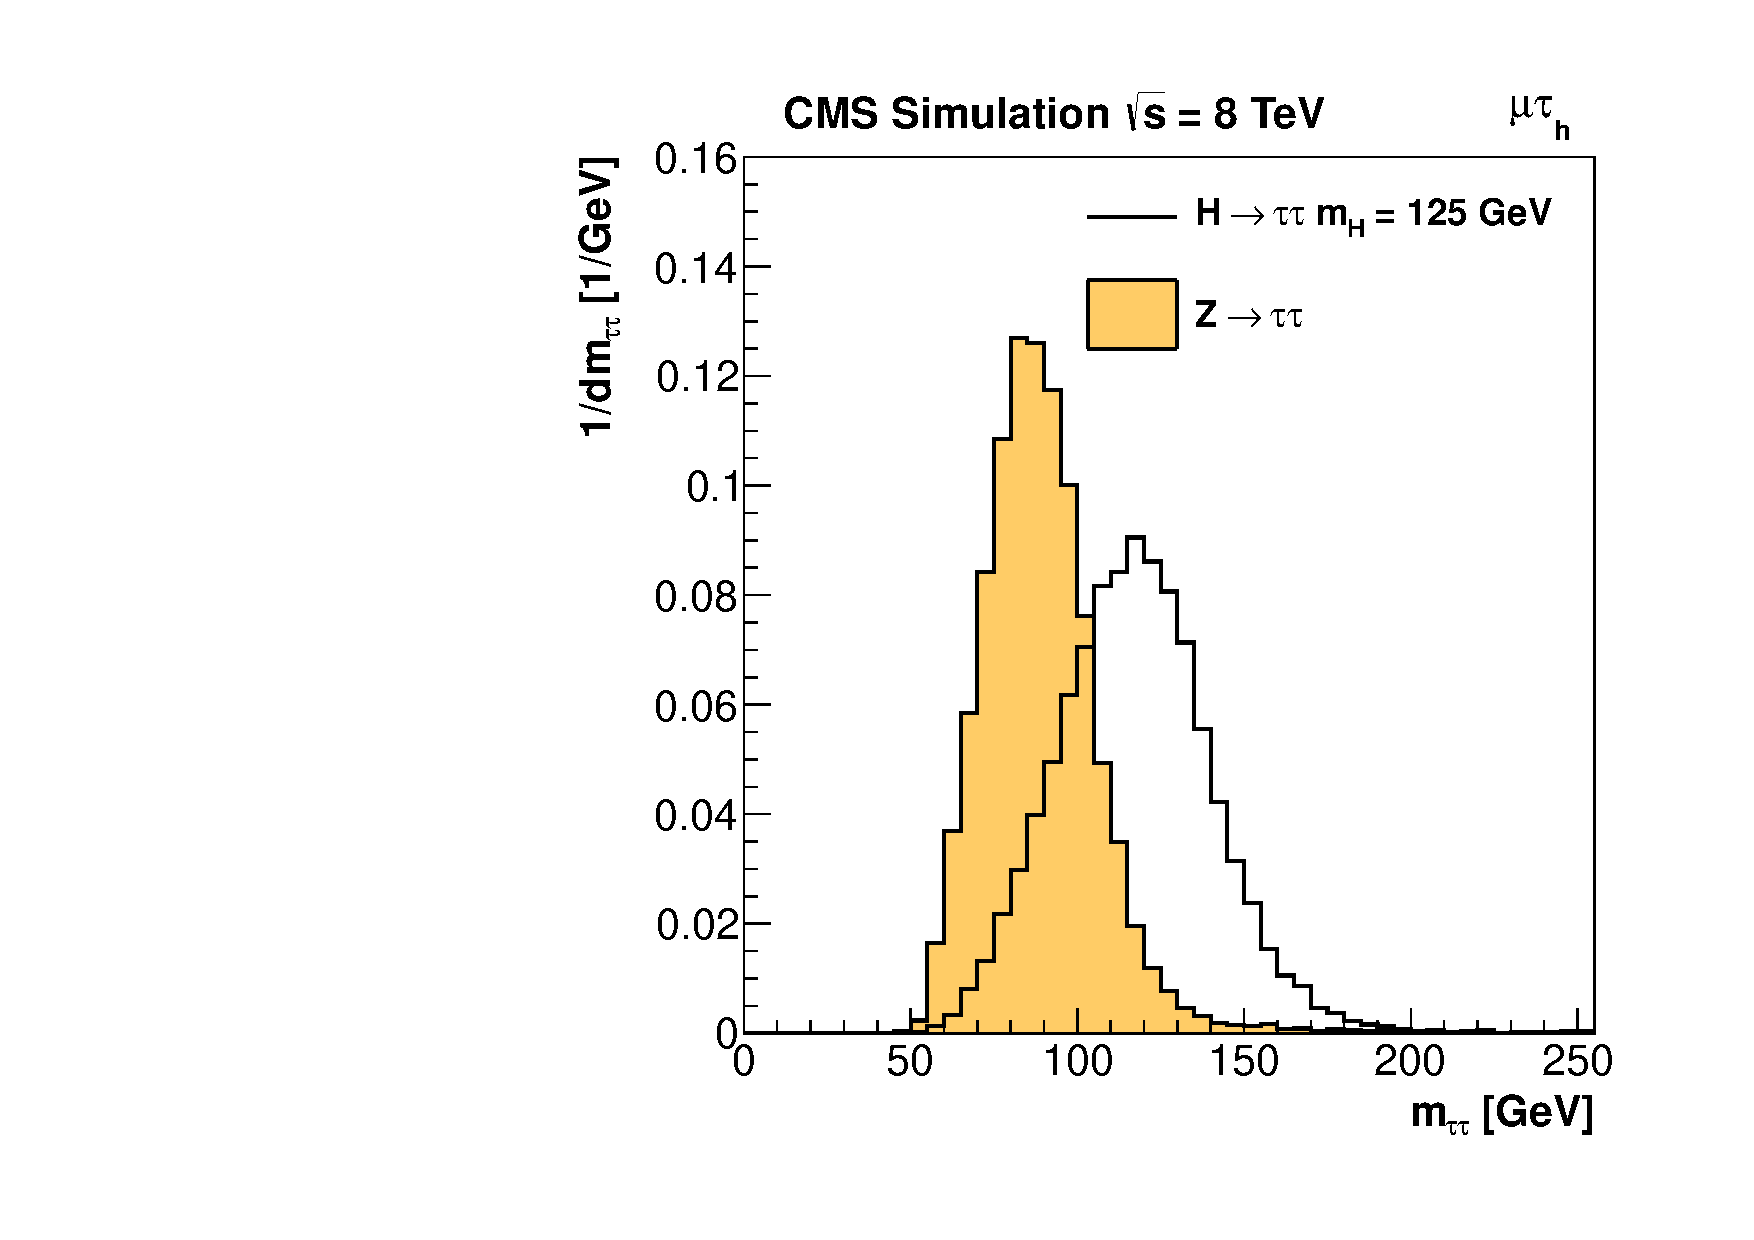
\includegraphics[width=0.5\textwidth] 
      {plots/reco/svFitPerformance_forColin_svFitMass.pdf}} 
\end{center}
\caption[Di-tau mass for for $\ZToTauTau$ and $\HToTauTau$ events, reconstructed
using the visible products or the SVFit algorithm.]{Visible di-tau (a) and SVFit
di-tau (b) mass for $\ZToTauTau$ and $\HToTauTau$ events \cite{HIG-13-004}.
} 
\label{fig:svfit}
\end{figure}

%\section{\ac{MC} simulation of signal and backgrounds}

%To model the contributions of signal and background events in the analysis
%Monte-Carlo (MC) simulation is used. Simulation of signal events is generated
%using POWHEG \cite{powheg} interfaced to PYTHIA \cite{pythia}, and of
%background events using MADGRAPH \cite{madgraph}. Pileup is simulated using
%additional interactions from PYTHIA and reweighting the simulated events to
%match the observed pileup distribution in data, which is different depending on
%the run period. In addition, the $E_{\rm{T}}^{\rm{miss}}$ response in
%simulation is corrected for the $E_{\rm{T}}^{\rm{miss}}$ energy scale and
%resolution which is measured in $Z\rightarrow\mu\mu$ events. The generated
%events are then processed through a simulation of the CMS detector based on
%GEANT4 \cite{geant4} and are reconstructed with the same algorithms used in
%data.



